\documentclass[../main.tex]{subfiles}
%!TEX root = ./chapter2ProposedDesign.tex
\graphicspath {{../}}

\begin{document}
\chapter{Proposed Design}
\section{Airship Envelope}
The airship design provided is for reference only as Dr. Lanteigne will be proceeding with his preferred design. The airship features hemispheres at each end, a cylinder attached to the front hemisphere and a cone bridging the gap from the cylinder and the rear hemisphere. The length of any section of the airship is limited to 5ft as that is the width of Dr. Lanteigne's polyurethane roll. The airship will feature fixed fins for stability during forward flight. A render of the full airship can be seen in Figure \ref{fig:fullAirship}. 

\begin{figure}[H]
	\centering
	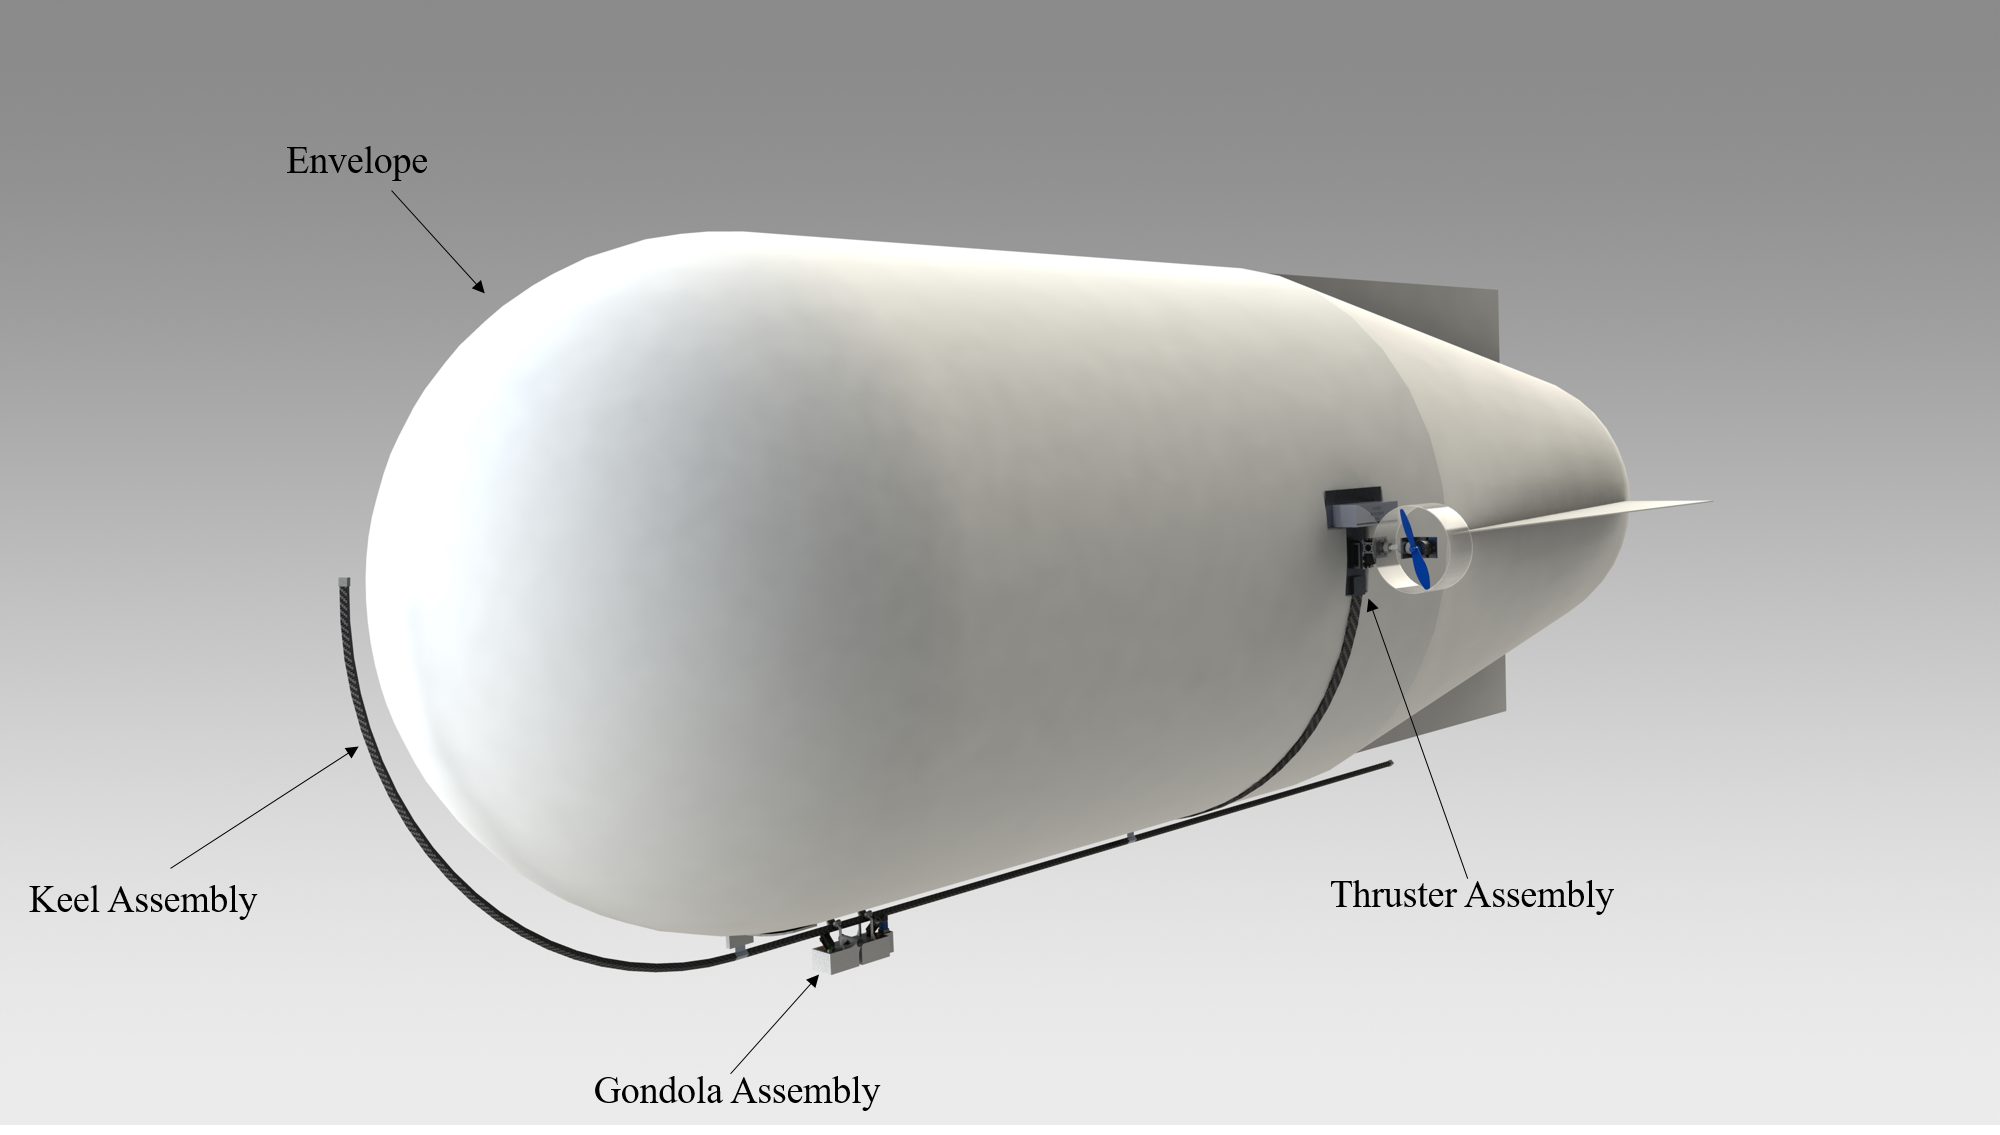
\includegraphics[width=\textwidth]{img/design/fullAirshipPerspective.png}
	\caption{Render of Full Airship Design}
	\label{fig:fullAirship}
\end{figure}

\section{Gondola}
The gondola sub-assembly is the most distinguishable feature of the airship design. The gondola moves along the keel in order to rapidly pitch the airship. The assembly can be seen in  Figure \ref{fig:gondolaIsomeric}. Movement along the gondola is initiated by two friction wheels which interface with the polyurethane cover on the keel through the friction between the two surfaces. Bearings are used as wheels to hold the gondola in position on the keel and facilitate sliding, while the friction wheels are in contact with the bottom edge of the keel. 

\begin{figure}[H]
	\centering
	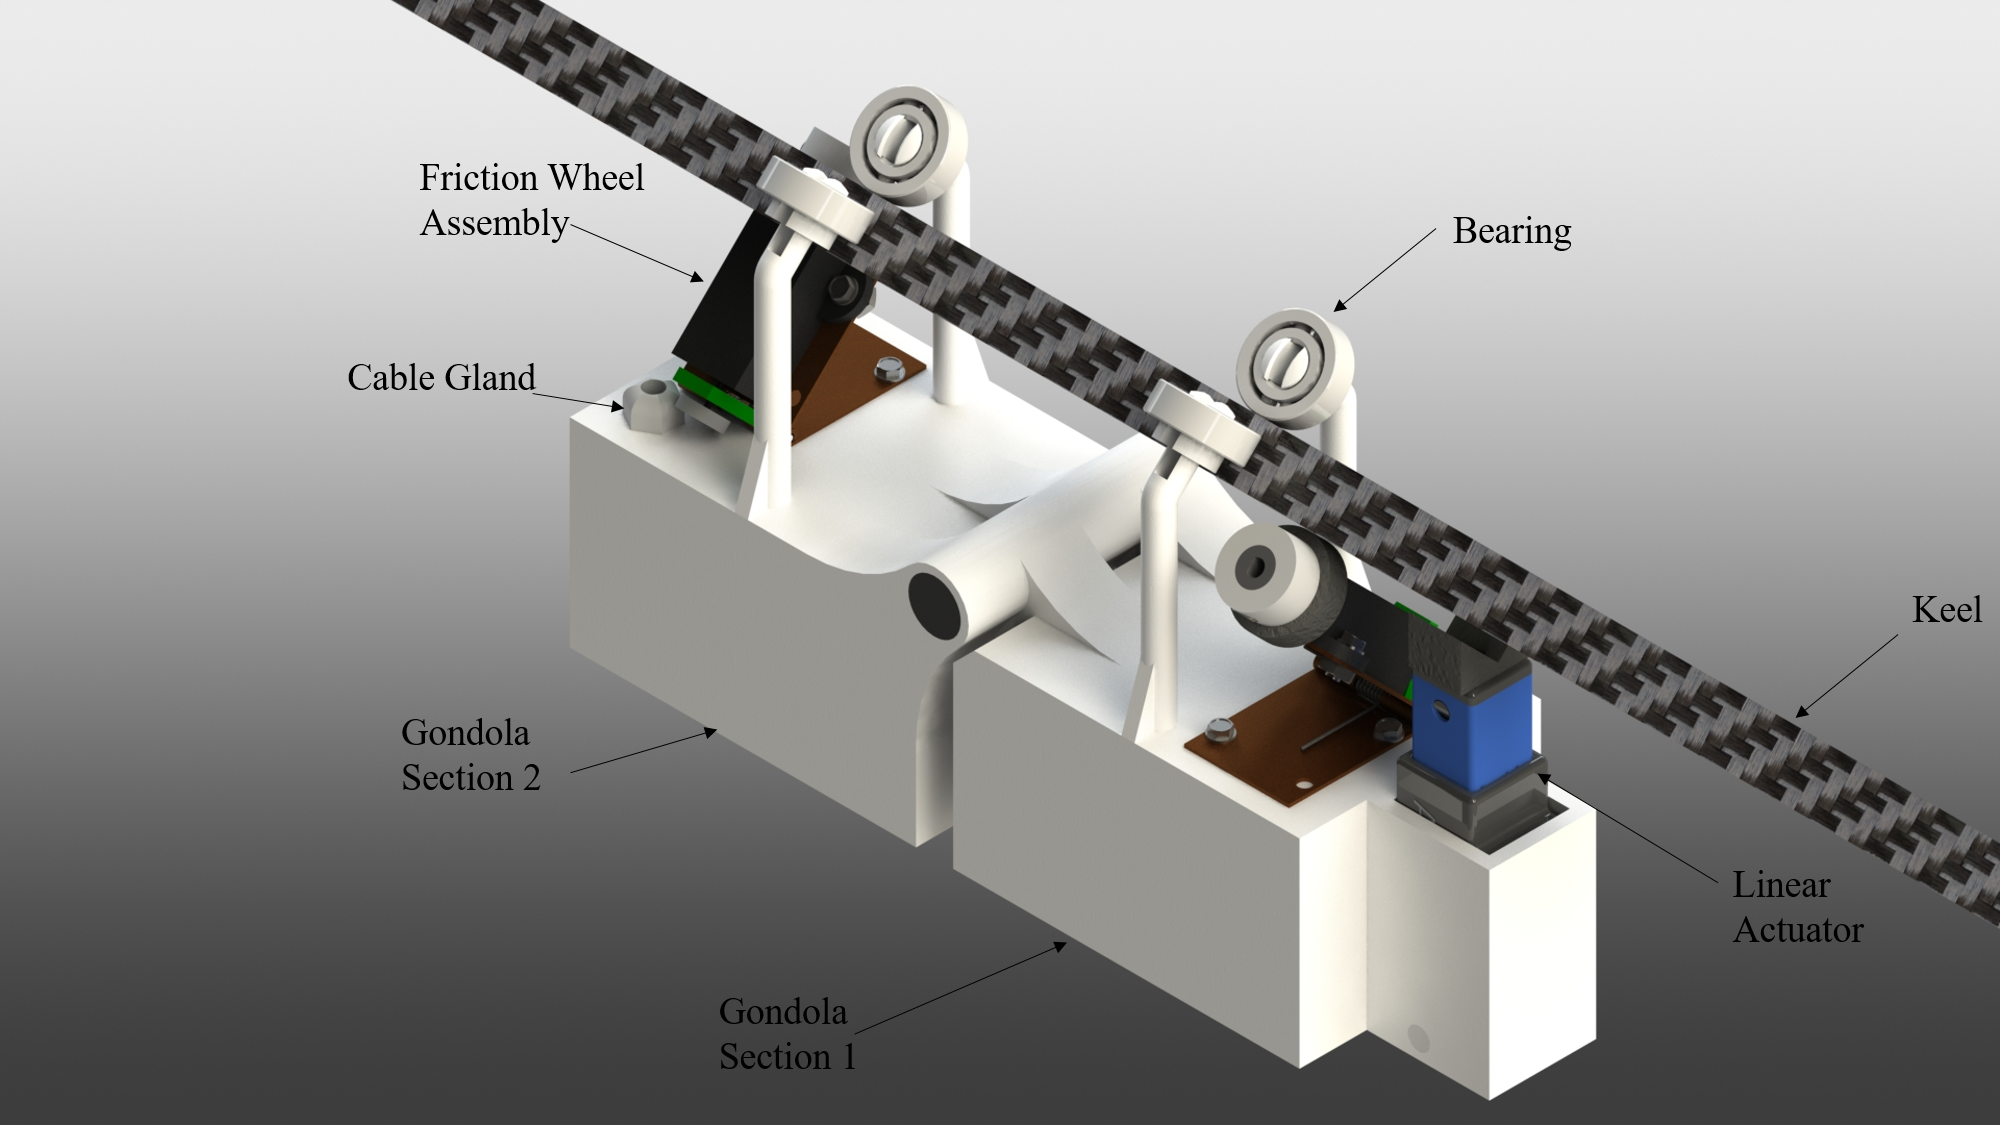
\includegraphics[width=.8\linewidth]{img/design/gondola/gondolaIsometric.png}
	\caption{Isometric View of the Gondola Assembly on the Keel}
	\label{fig:gondolaIsomeric}
\end{figure}

The gondola is comprised of two half sections, each housing required flight components: the battery, flight controller, transmitter, GPS module and two ESCs. Figure \ref{fig:gondolaPartialSection} shows how these components are nested in one of the gondola sections. 

\begin{figure}[H]
	\centering
	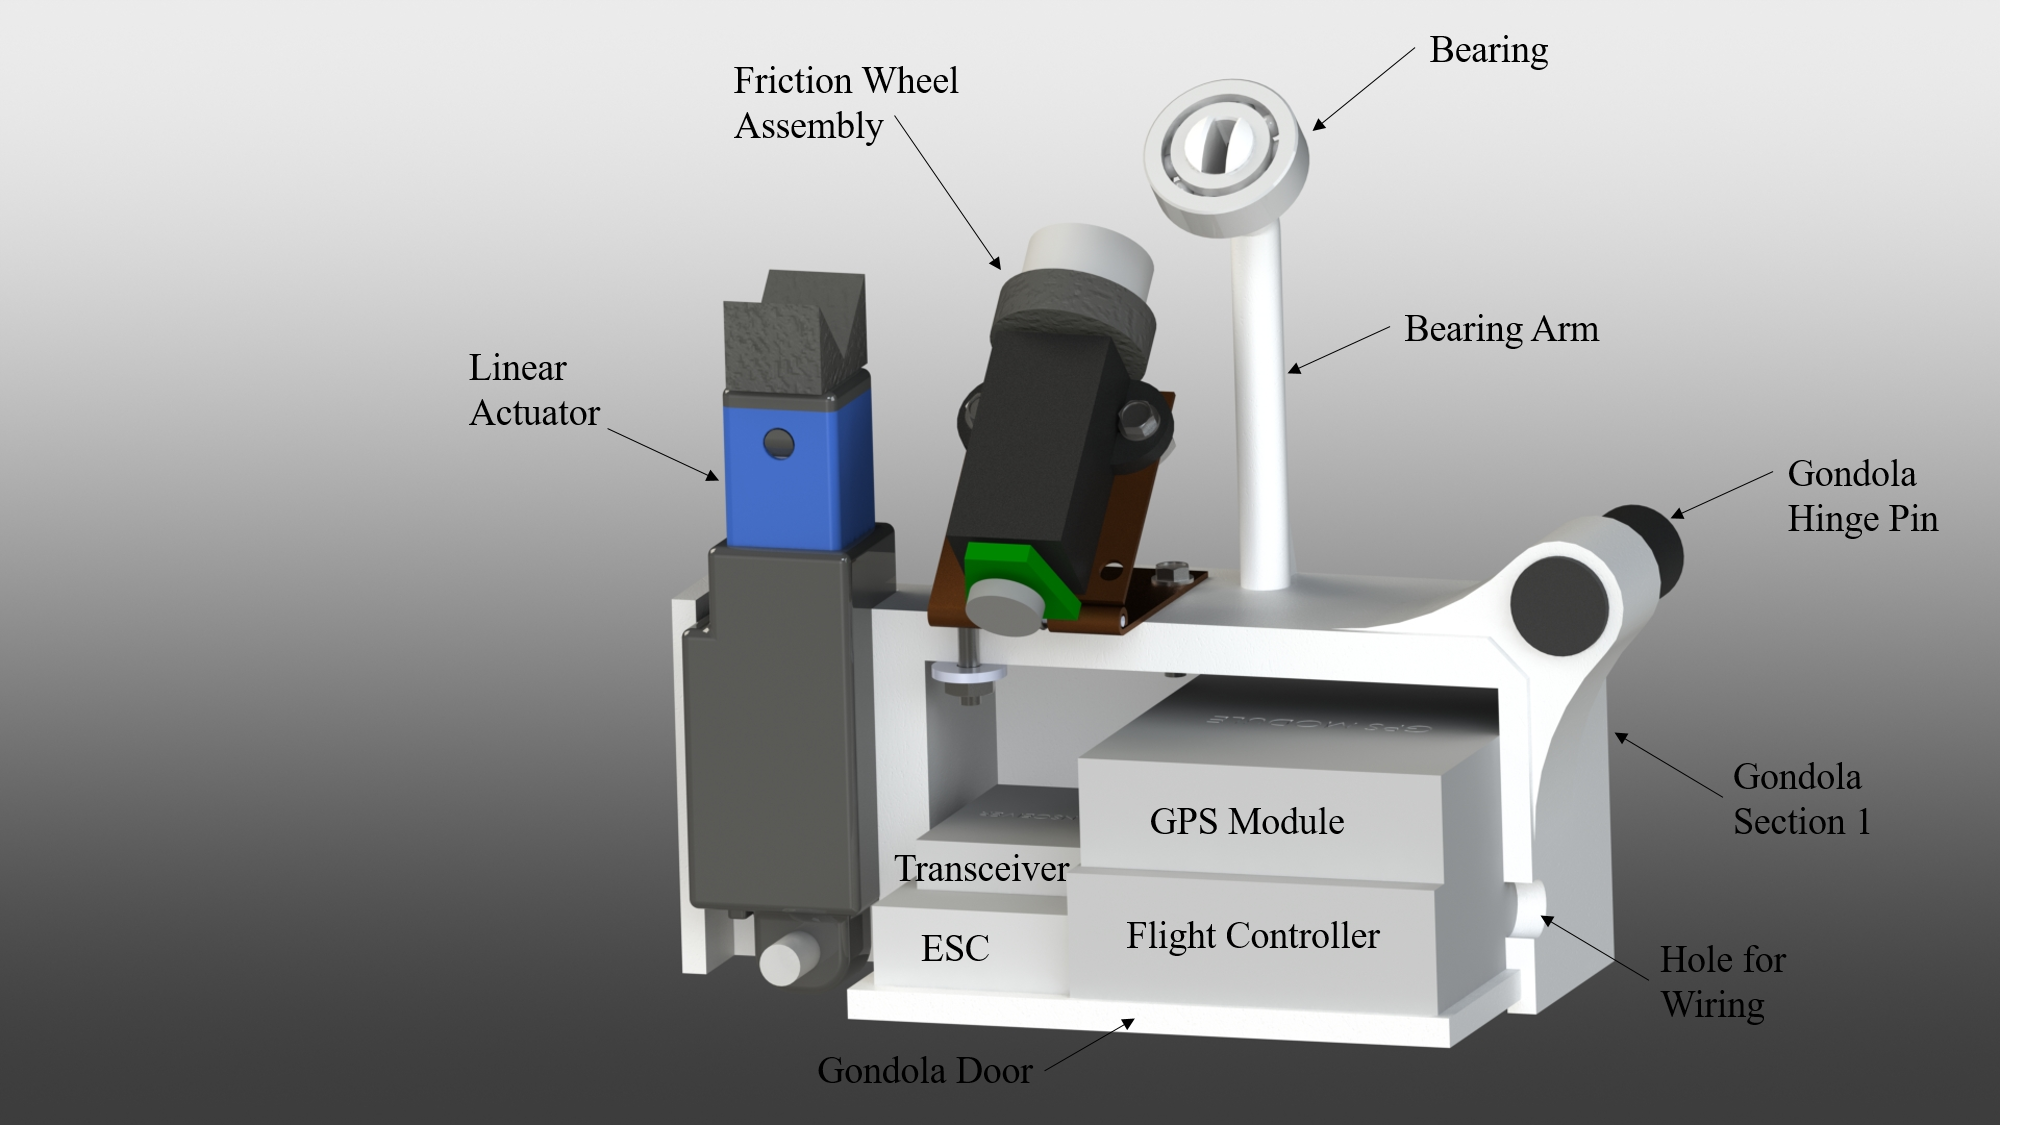
\includegraphics[width=.8\linewidth]{img/design/gondola/gondolaPartialSection.png}
	\caption{Partial Section of Gondola 1 (Components)}
	\label{fig:gondolaPartialSection}
\end{figure}

A hinge joins the two sections, as seen in Figure \ref{fig:gondola1ExplodedView}, which allows the gondola to bend freely in the centre. The hinge has a flanged end and a cap that relies upon an interference fit to ensure the hinge does not slip out of the gondola axially. The bend in the middle allows the gondola to overcome a more significant turning radius compared to being fixed in a straight line, which is depicted in Figure \ref{fig:gondolaBent}. Similarly to curve fitting, the more points that are used, the better fit. 

\begin{figure}[H]
	\centering
	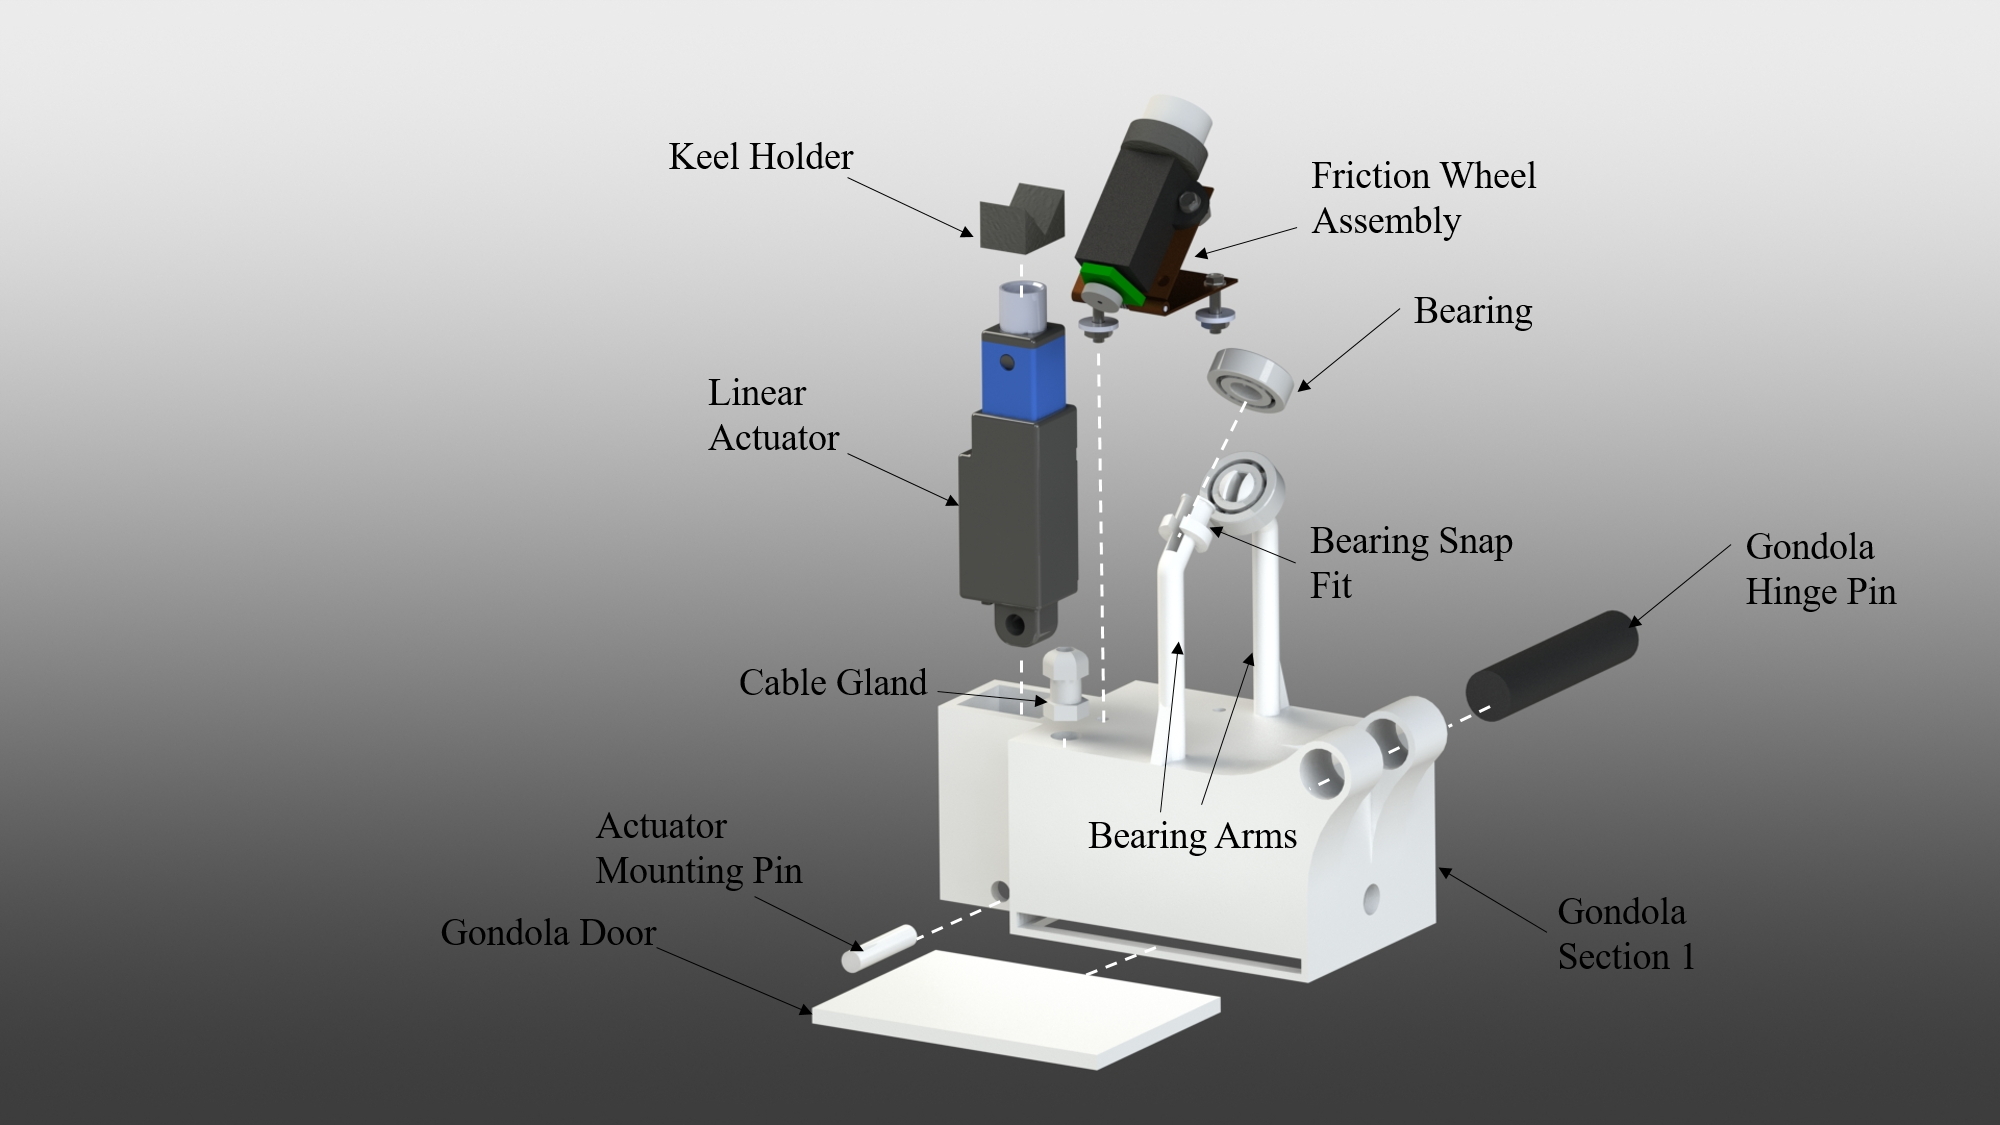
\includegraphics[width=.8\linewidth]{img/design/gondola/gondola1ExplodedView.png}
	\caption{Gondola 1 Exploded View}
	\label{fig:gondola1ExplodedView}
\end{figure}

\begin{figure}[H]
	\centering
	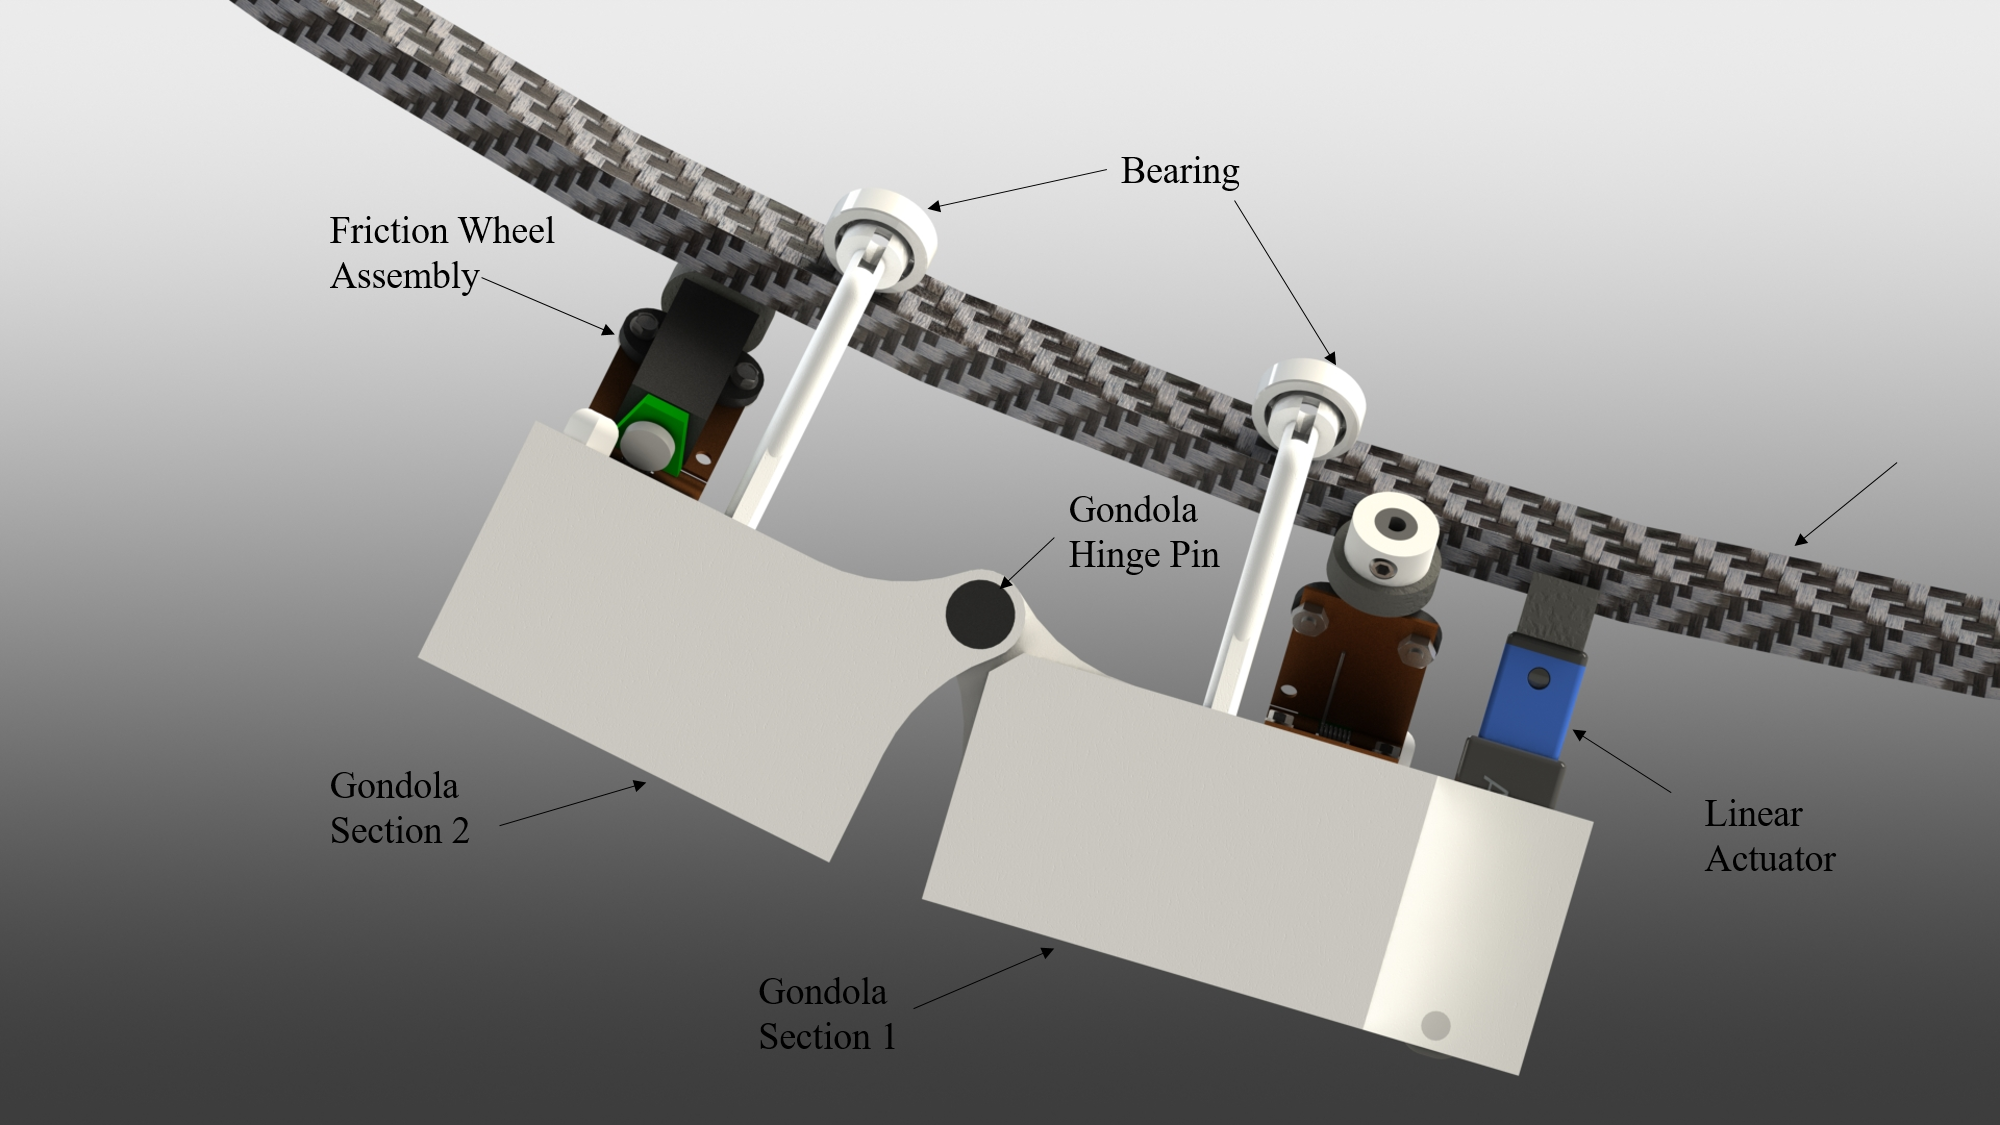
\includegraphics[width=.8\linewidth]{img/design/gondola/gondolaBent.png}
	\caption{Gondola Assembly on Curved Section of Keel}
	\label{fig:gondolaBent}
\end{figure}

Braking of the gondola is accomplished by turning the friction wheels in the opposite direction until motion is stopped. Once this occurs, the position is held by a linear actuator, which provides force perpendicular to the keel surface. The linear actuator motion can be seen in Figure \ref{fig:linearActuatorAndMotor}. The gondola has been designed to be resistant to small amounts of water, considering the gondola will always be shielded from rainfall by the envelope, therefore less waterproofing is required. Cable glands (see Appendix \ref{CableGland}) will be used for all surfaces perpendicular to rainfall that require waterproofing. They can be seen more clearly in Figure \ref{fig:gondola1ExplodedView}. The gondola sections are made using high quality 3D prints, given their complex geometries and relatively small size.
\\

\begin{figure}[H]
	\centering
	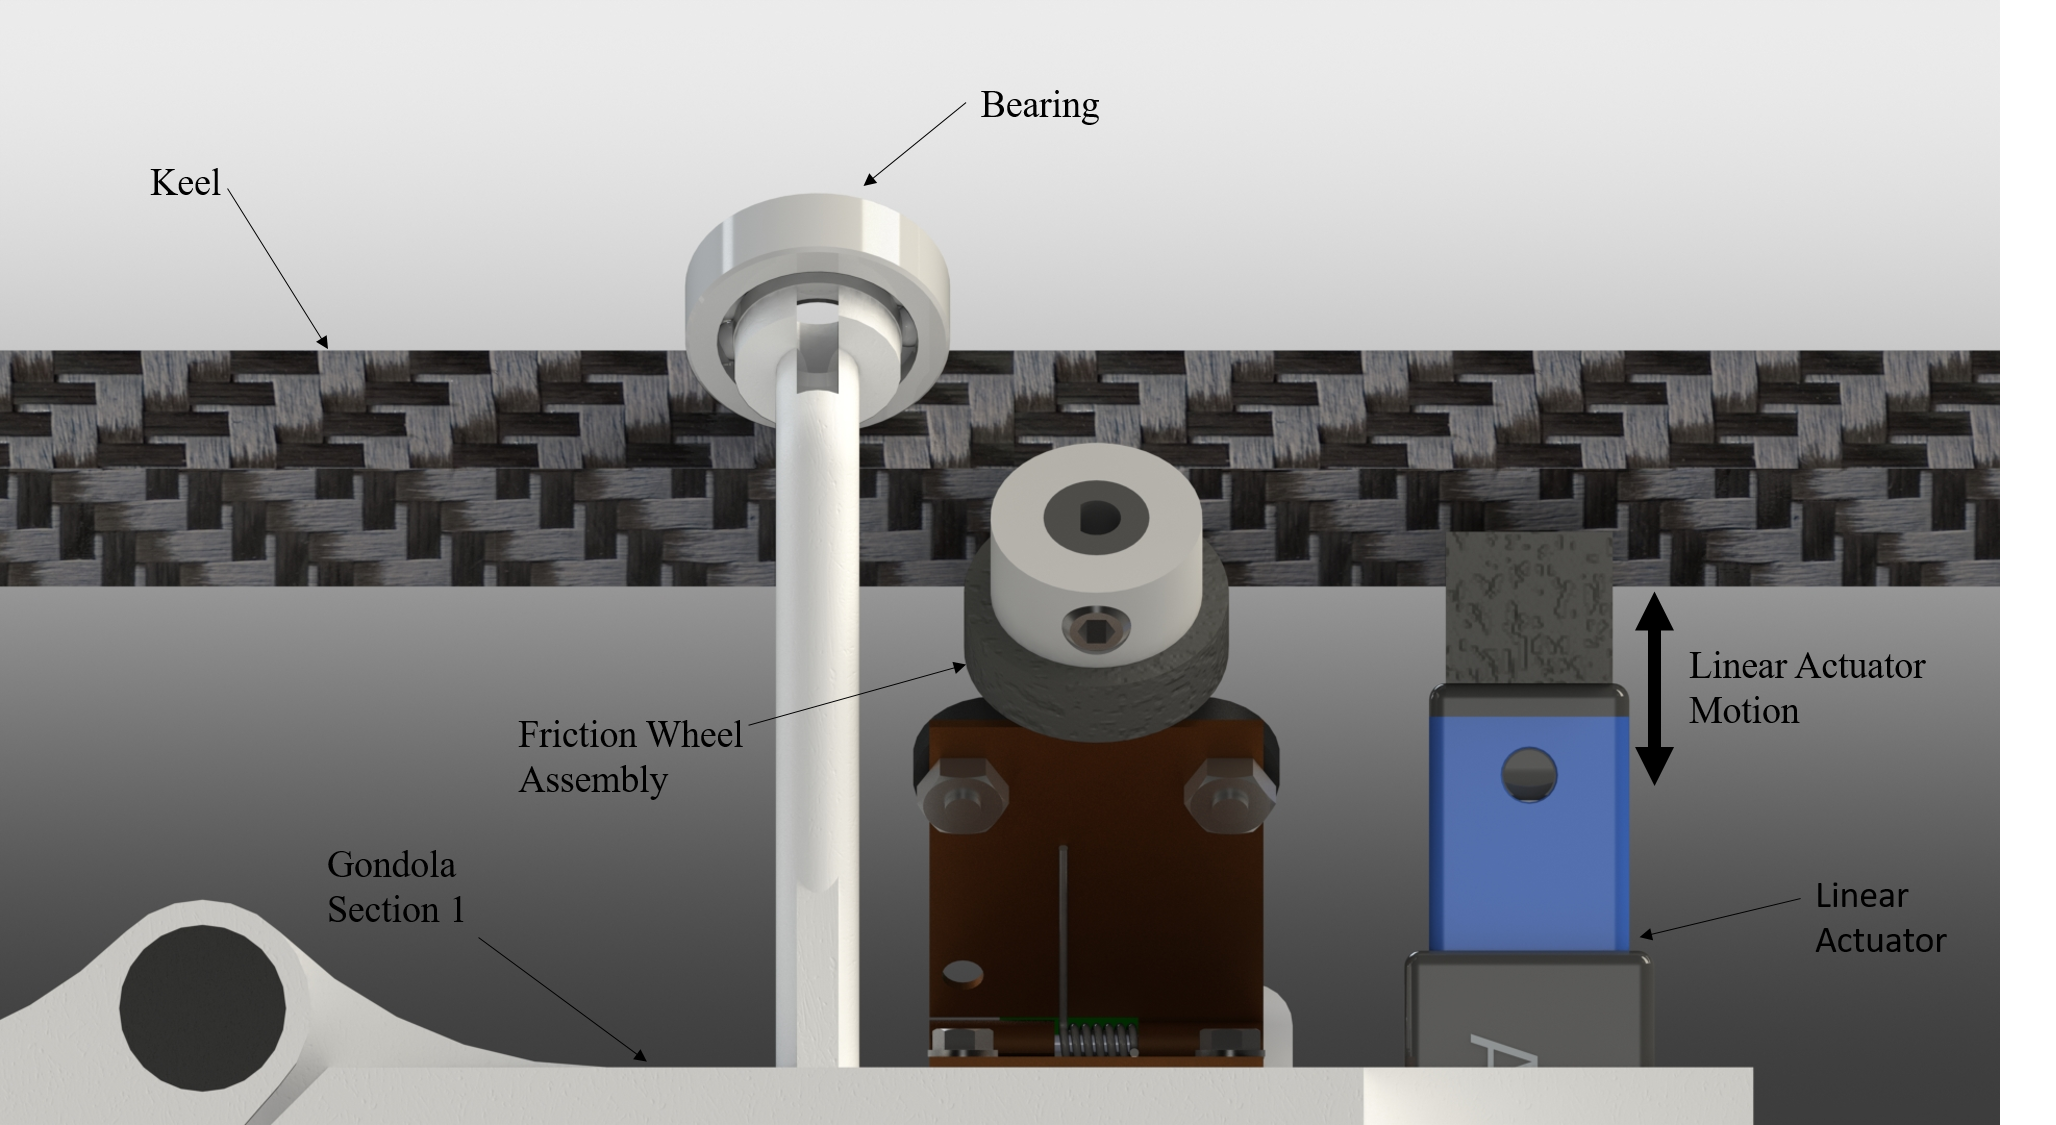
\includegraphics[width=.8\linewidth]{img/design/gondola/linearActuatorAndMotor.png}
	\caption{Linear Actuator Motion}
	\label{fig:linearActuatorAndMotor}
\end{figure}

\subsection{Friction Wheel}
The friction wheel must always be in contact with the keel, shown in Figure \ref{fig:frictionWheelOnGondola}. The friction wheel is made from 55D rubber, purchased off-the-shelf. It has a shore hardness of 55A, which is considered medium soft, so it can deform when it is placed on the keel. A shaft adapter is necessary to bridge the gap between the motor shaft and the friction wheel, as the two sizes are not compatible. The shaft adapter will be 3D printed, and held in place by an existing set screw in the friction wheel. To ensure adequate pressure on the keel, the friction wheel assembly is mounted on a hinged bracket equipped with a torsion spring at the pin, as seen in Figure \ref{fig:explodedFrictionWheel}. The motor used can rotate in both directions, making it useful as a reverse rotating brake as well. A magnetic encoder allows for accurate positioning of the gondola sections, independently allowing for redundancy between the two motors. The motor is mounted to the bracket using two nuts and two bolts. The bracket is mounted to the gondola using 2 nuts, 2 bolts and 2 washers. The hinged bracket will be manufactured in house with aluminium, and a sourced torsion spring (see Appendix \ref{TORSIONSPRING}).

\begin{figure}[H]
	\centering
	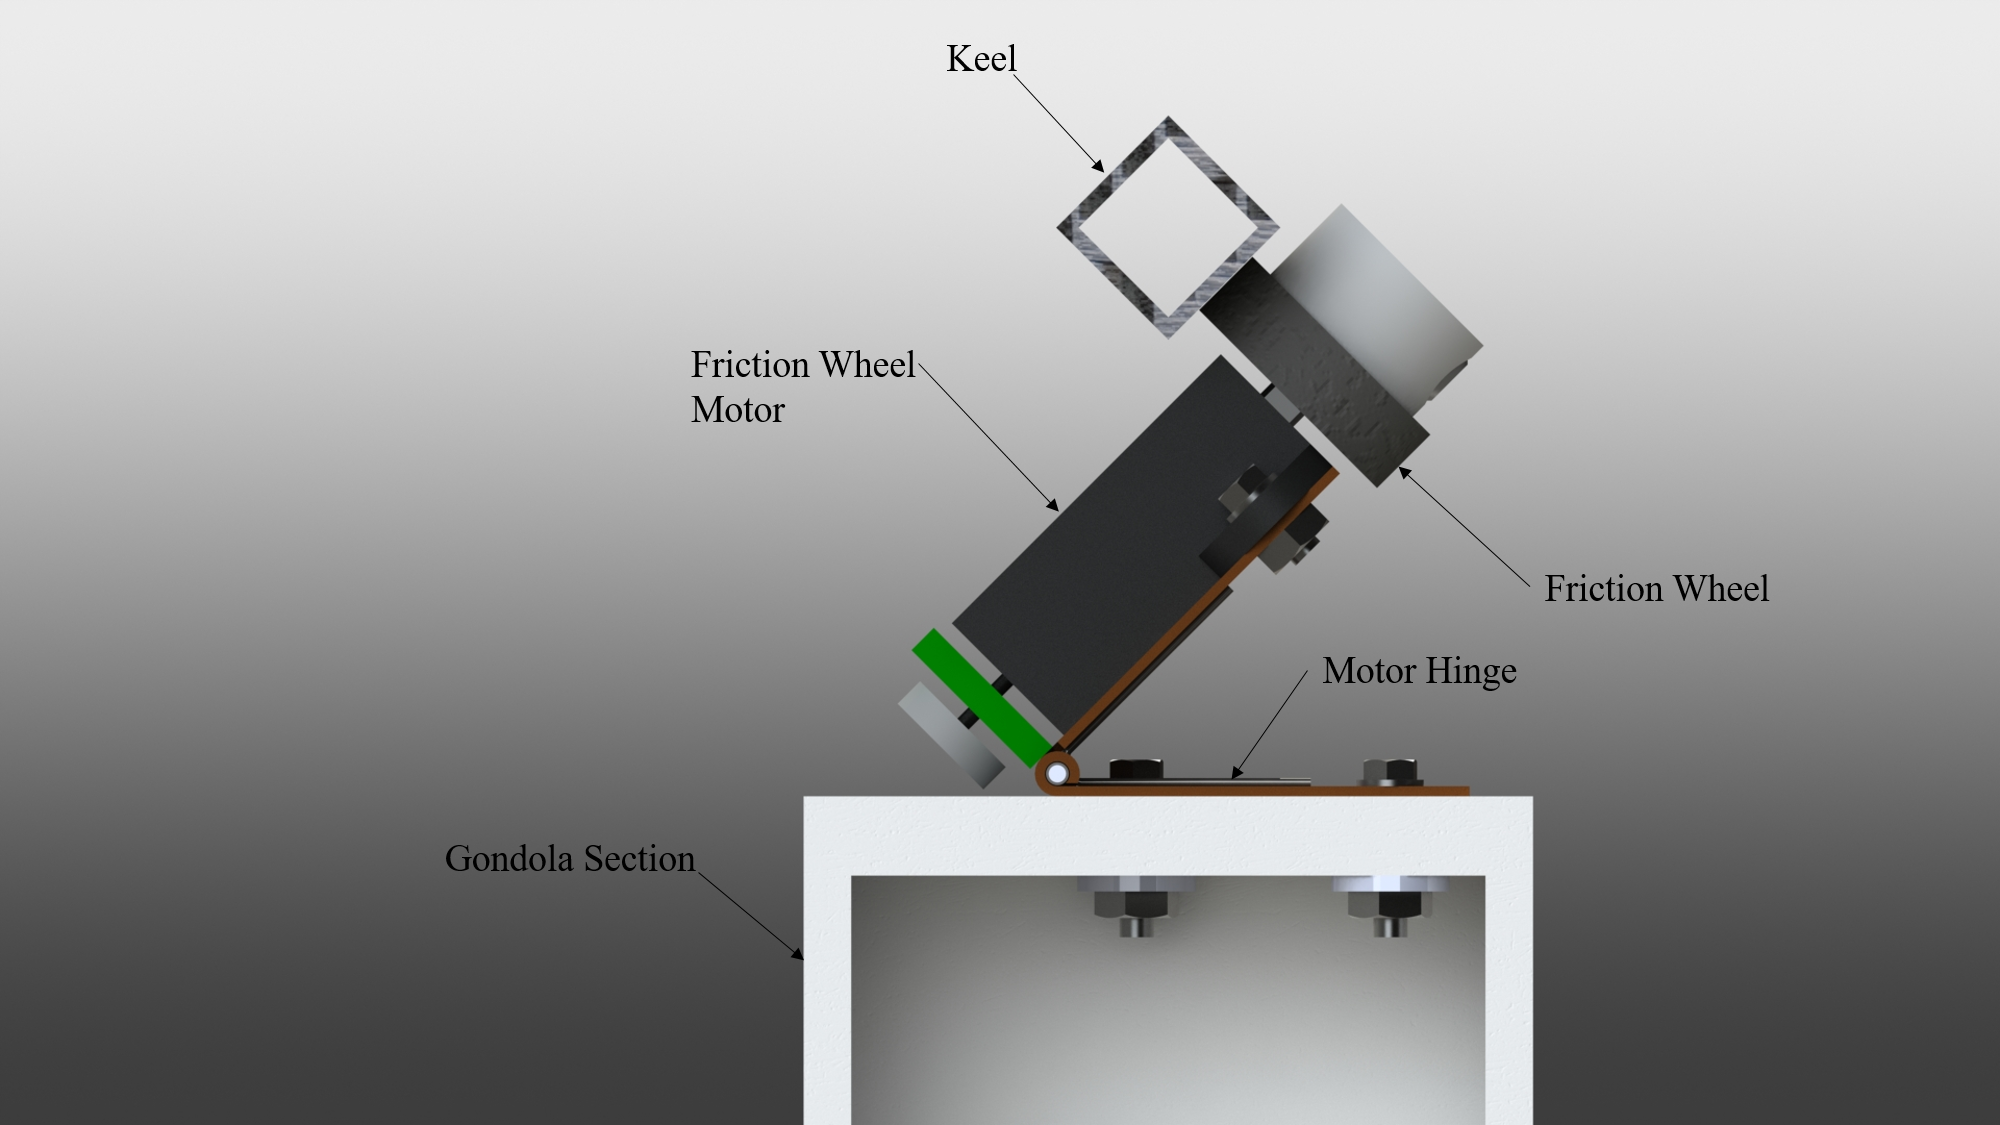
\includegraphics[width=.8\linewidth]{img/design/gondola/frictionWheelOnGondola.png}
	\caption{Friction Wheel Interfacing with the Keel}
		\label{fig:frictionWheelOnGondola}
\end{figure}
\begin{figure}[H]
	\centering
	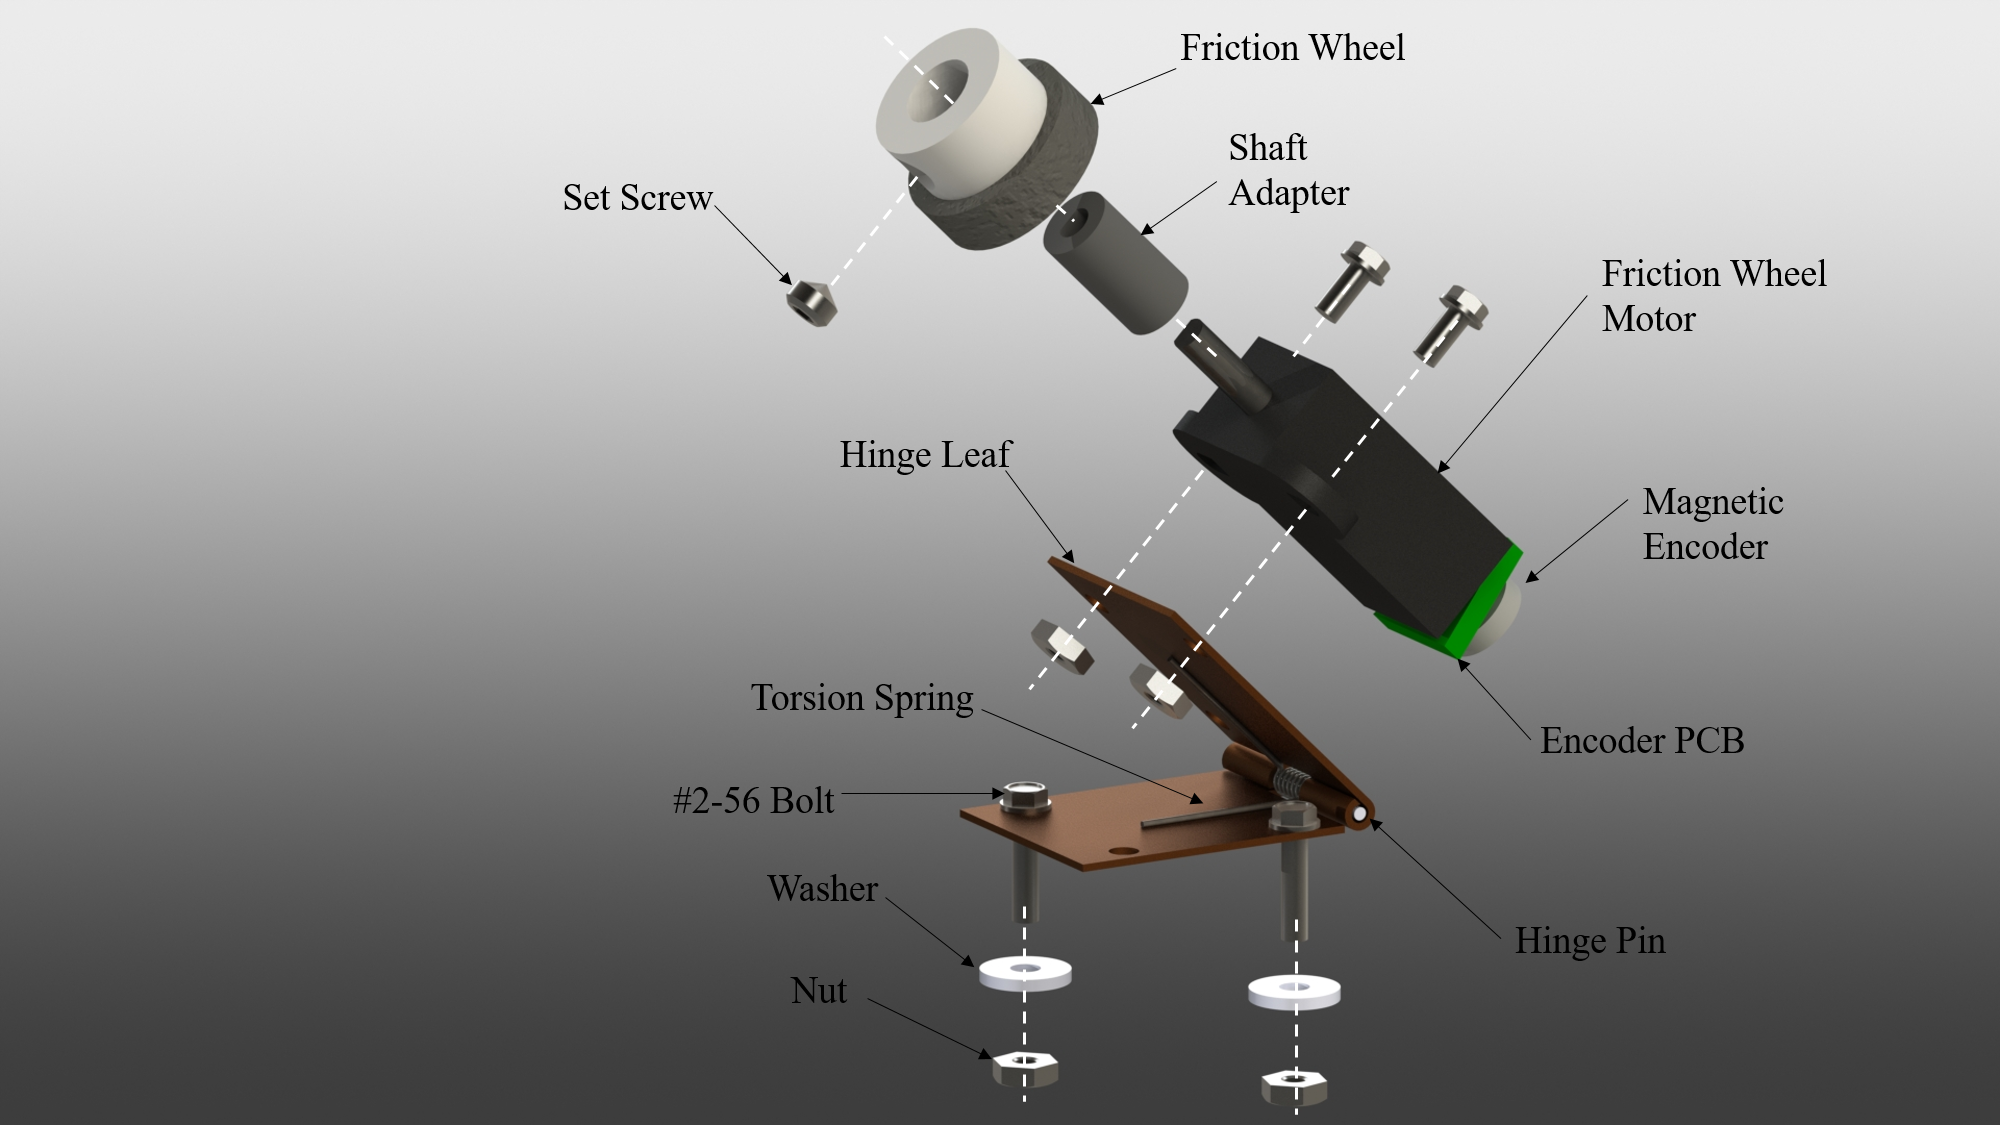
\includegraphics[width=.8\linewidth]{img/design/gondola/explodedFrictionWheel.png}
	\caption{Exploded View of the Friction Assembly}
	\label{fig:explodedFrictionWheel}
\end{figure}

\subsection{Bearings}
Bearings (Appendix \ref{PBearings}) are placed on top of the keel to support the weight of the gondola and counter the force applied to the keel by the friction wheel. The bearings act as wheels turning and slipping along the keel. Low weight, plastic bearings will be used. The bearings are mounted using a snap fit design, that can be seen in Figure \ref{fig:gondola1ExplodedView}. This bearing is held in place by a shaft diameter slightly larger than the bearing inner diameter. The bearing is placed over the piece, deflecting it until the bearing can slip past the overhang where the snap fit piece elastically snaps back into its original position, securely holding the bearing.
\\
\subsection{Linear Actuator}
A linear actuator is housed on one of the two sections of the gondola. The linear actuator is to be activated when the gondola is not moving to hold its position on the keel. The motion can be seen in Figure \ref{fig:linearActuatorAndMotor}. A custom 3D printed piece is outfitted to the top of the actuator (Keel Holder) in a V-shape to mesh ideally with the keel, as seen in Figure \ref{fig:gondola1ExplodedView}. The V-shaped 3D printed surface will then be coated with a Plasti Dip\textregistered{} like coating, to reduce the likelihood of tearing the polyurethane cover on the keel.  The  linear actuator chosen has a variety of holding forces without constant power, making it ideal for run time. It is also water resistant to the IP54 standard. 
\\
\subsection{Door and Components}
The gondola features a sliding door (the motion can be seen in Figure \ref{fig:gondola1ExplodedView}), to ease the process of component charging and changing. The door relies upon an interference fit to stay in place. Components are inserted into the gondola while it is off the keel and secured by double sided tape. The door is inserted and the gondola is reinserted onto the keel. See Figure \ref{fig:gondolaPartialSection} (selective cross-section). The door will also be 3D printed.
\\
\section{Keel}
Figure \ref{fig:keelAssemblyCompressedThruster} shows the keel assembly in a condensed form. The two straight and one curved sections of the keel and the envelope support originate from Dr. Lanteigne's design. Sections of the keel are joined using connectors that rely on interference fits, also designed by Dr. Lanteigne. The connectors are modified and machined for improved material properties. The proposed design involves much higher forces applied to the connector pieces than the previous design. 

\begin{figure}[H]
	\centering
	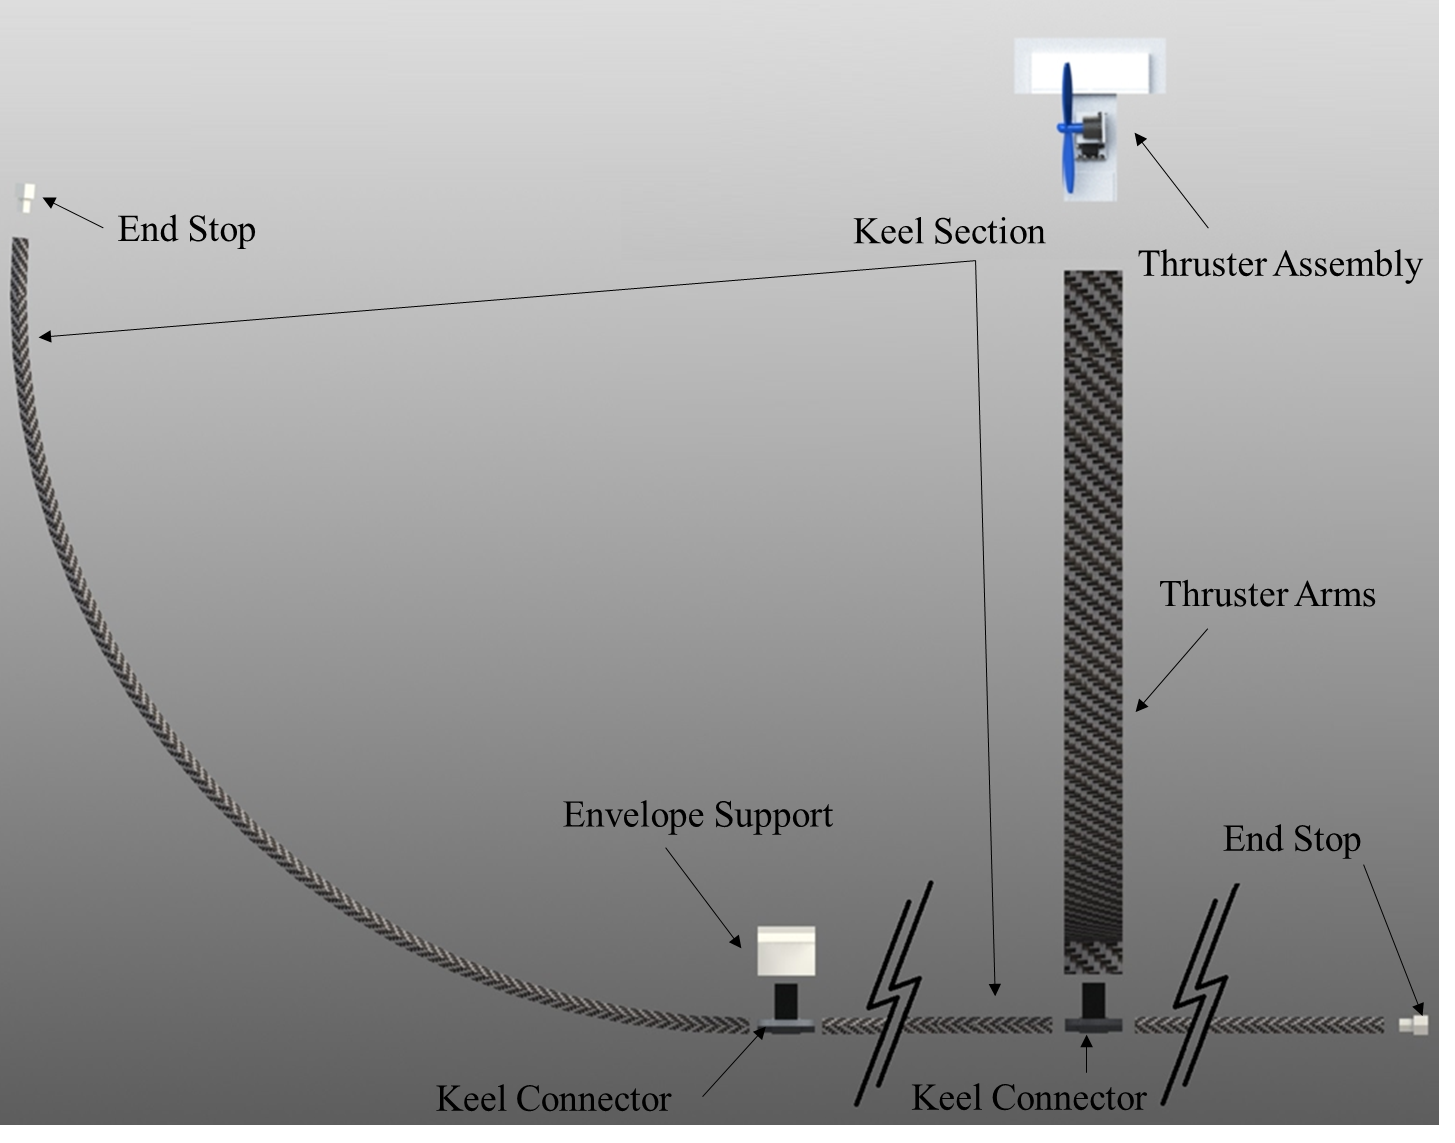
\includegraphics[width=.8\linewidth]{img/design/keel/keelAssemblyCompressedThruster.png}
	\caption{Overall Keel Assembly (Compressed)}
	\label{fig:keelAssemblyCompressedThruster}
\end{figure}

The envelope support slides into a slot on the keel connectors remaining in position by bottoming out. The surface will also be lathered with epoxy to prevent the piece from falling out when the airship is perpendicular to the ground (see Appendix \ref{adhesion} for adhesion calculations). Thrusters are mounted on carbon fibre arms that also slide into the connector, maintaining position by bottoming out and epoxy as well. The section shown in Figure \ref{fig:thrusterArmConnectorCrossSection} displays the bottoming out and Figure \ref{fig:thrusterArmConnectorPiece} shows the fit.

\begin{figure}[H]
	\centering
	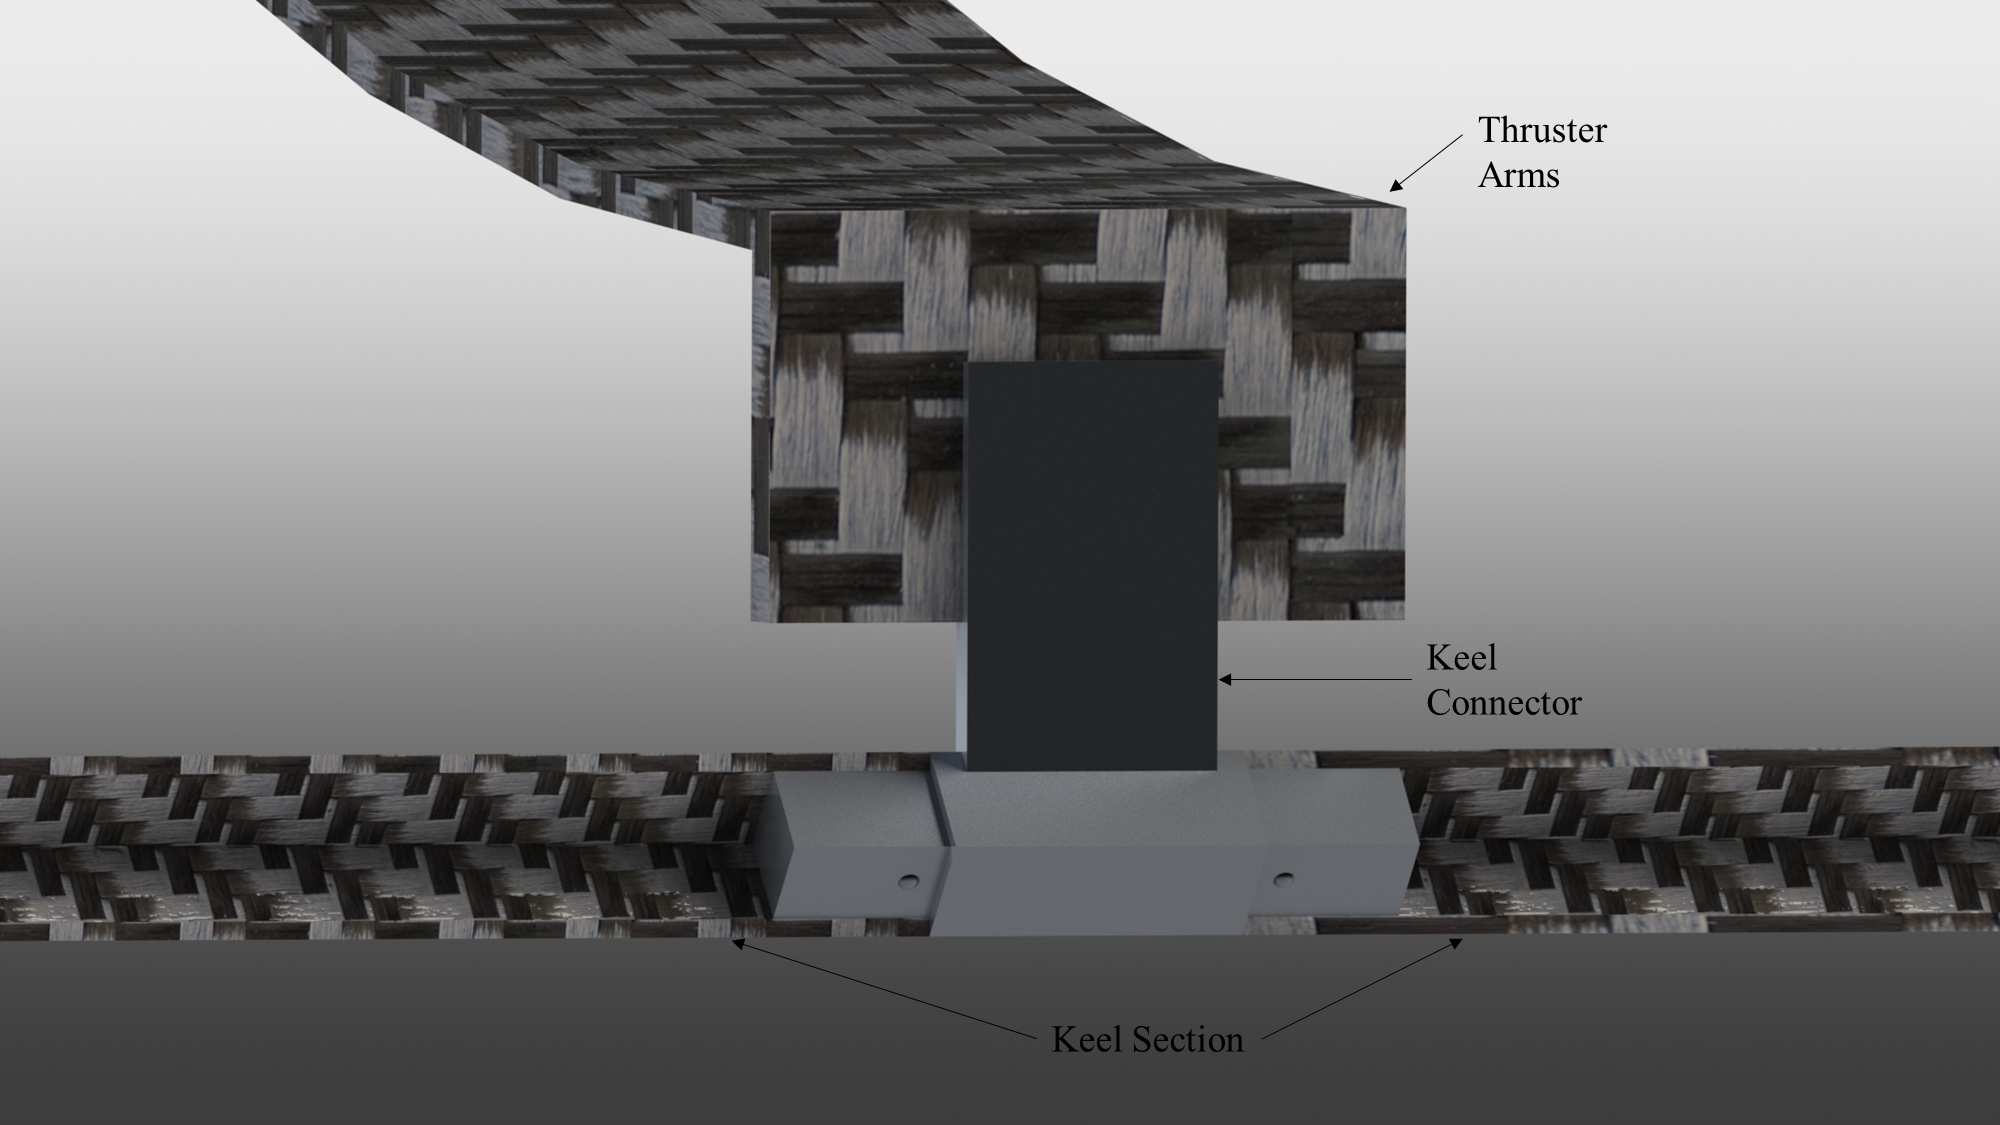
\includegraphics[width=.9\linewidth]{img/design/keel/thrusterArmConnectorCrossSection.png}
	\caption{Cross-Section of the Keel Connector}
	\label{fig:thrusterArmConnectorCrossSection}
\end{figure}
\begin{figure}[H]
	\centering
	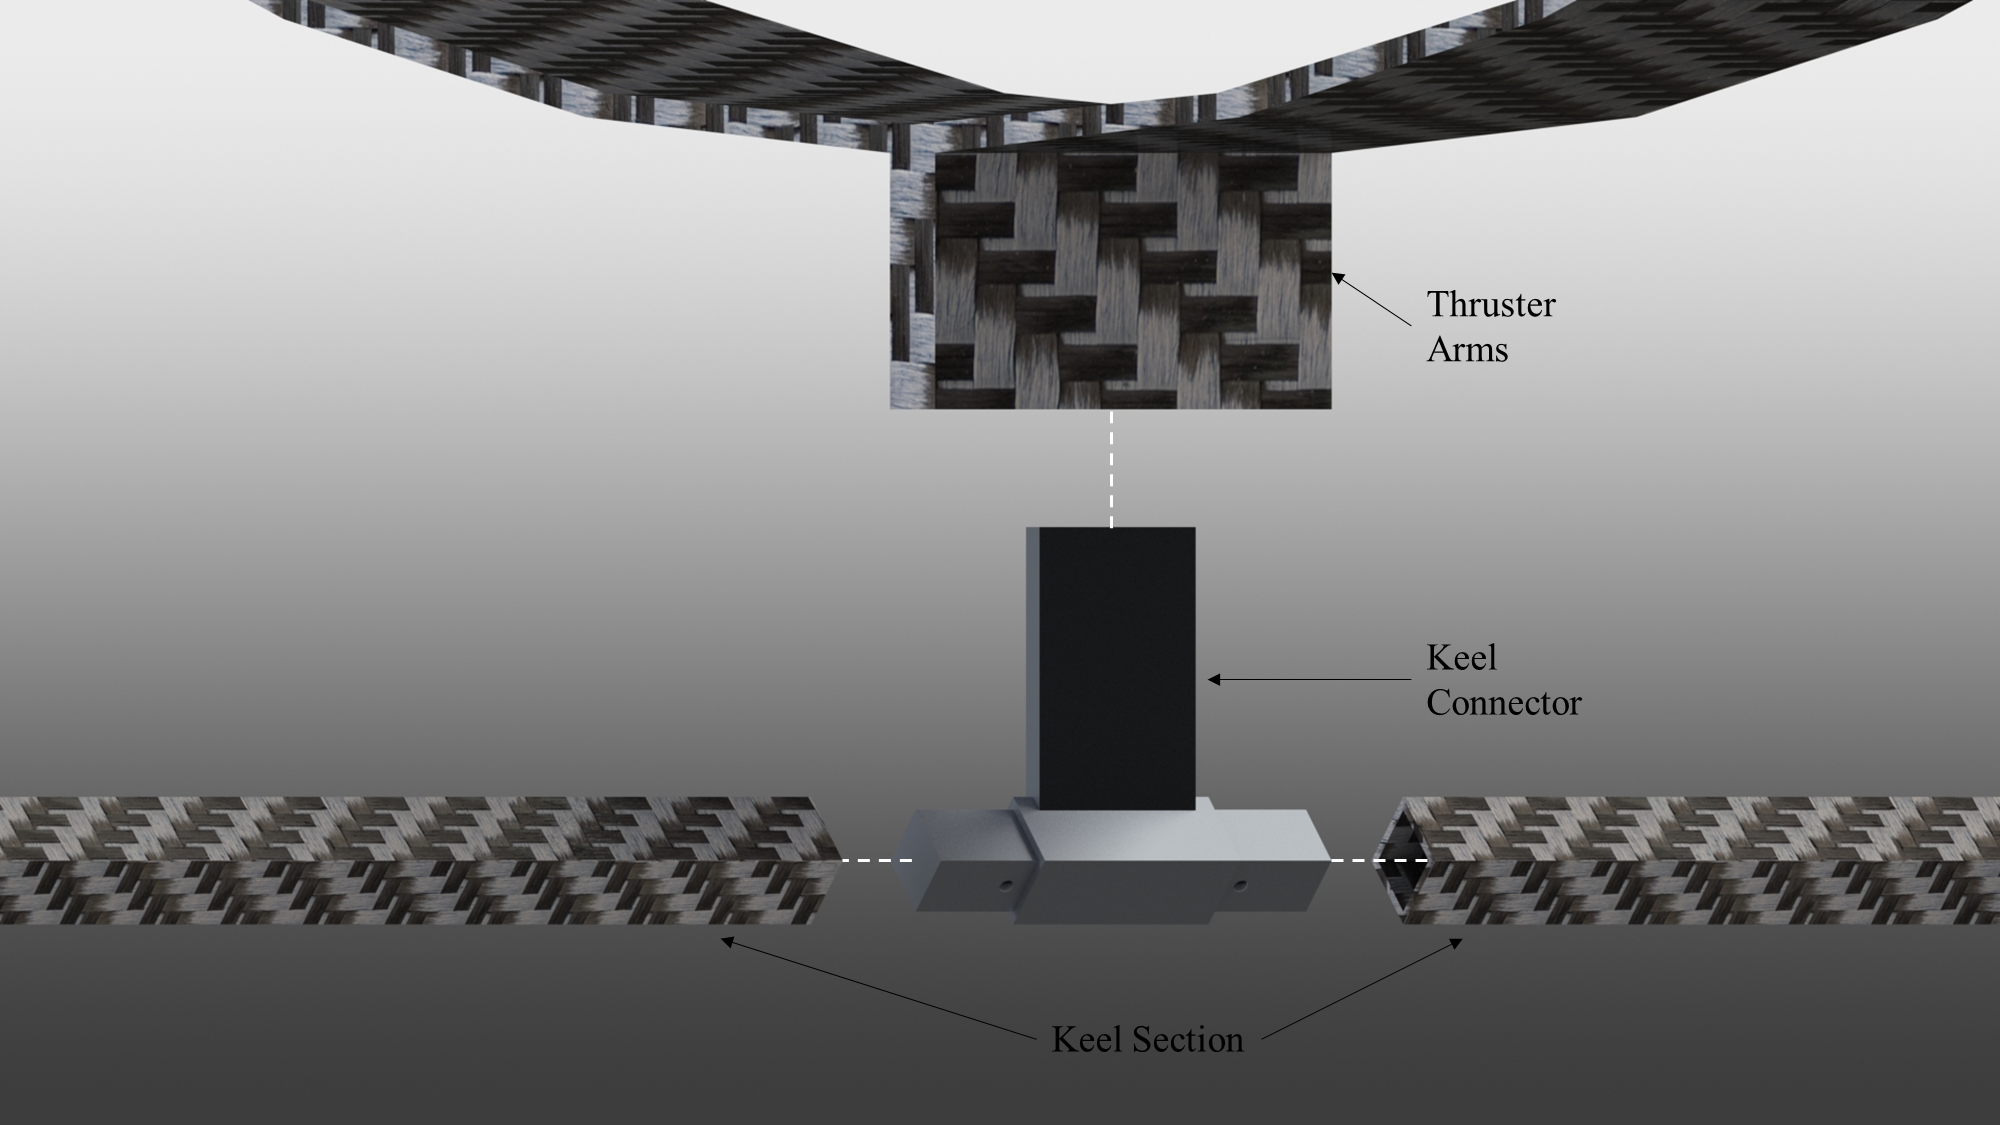
\includegraphics[width=.9\linewidth]{img/design/keel/thrusterArmConnectorPiece.png}
	\caption{Connector Piece Assembling}
	\label{fig:thrusterArmConnectorPiece}
\end{figure}

 3D printed end stops are inserted in either end of the keel using an interference fit identical to the connectors. The end stop design can be seen in Figure \ref{fig:keelEndCap}. The stops are slightly larger than the size of the keel, effectively interfering with the gondola friction wheels, thereby keeping the gondola from rolling off the ends of the keel. All geometries in the keel assembly are fixed in relation to the airship with the exception of the thrusters.

\begin{figure}[H]
	\centering
	\includegraphics[width=.8\linewidth]{img/design/keel/keelEndCap.png}
	\caption{Keel End Stop}
	\label{fig:keelEndCap}
\end{figure}


\subsection{Thrusters}
The thruster arms are made from carbon fibre that will be made in house by laying sheets of carbon fibre on a balloon mould. A CNC machined aluminium plate is attached to the U-shaped carbon fibre arms by welding a machined cap piece onto the plate, then inserting the carbon fibre arm into it and applying epoxy. The aluminium plate and bearing arms are built in a way that will interfere with the airship, causing compression of the helium and polyurethane sheet. This compression is shown in Figure \ref{fig:envelopeDeformation}.

\begin{figure}[H]
	\centering
	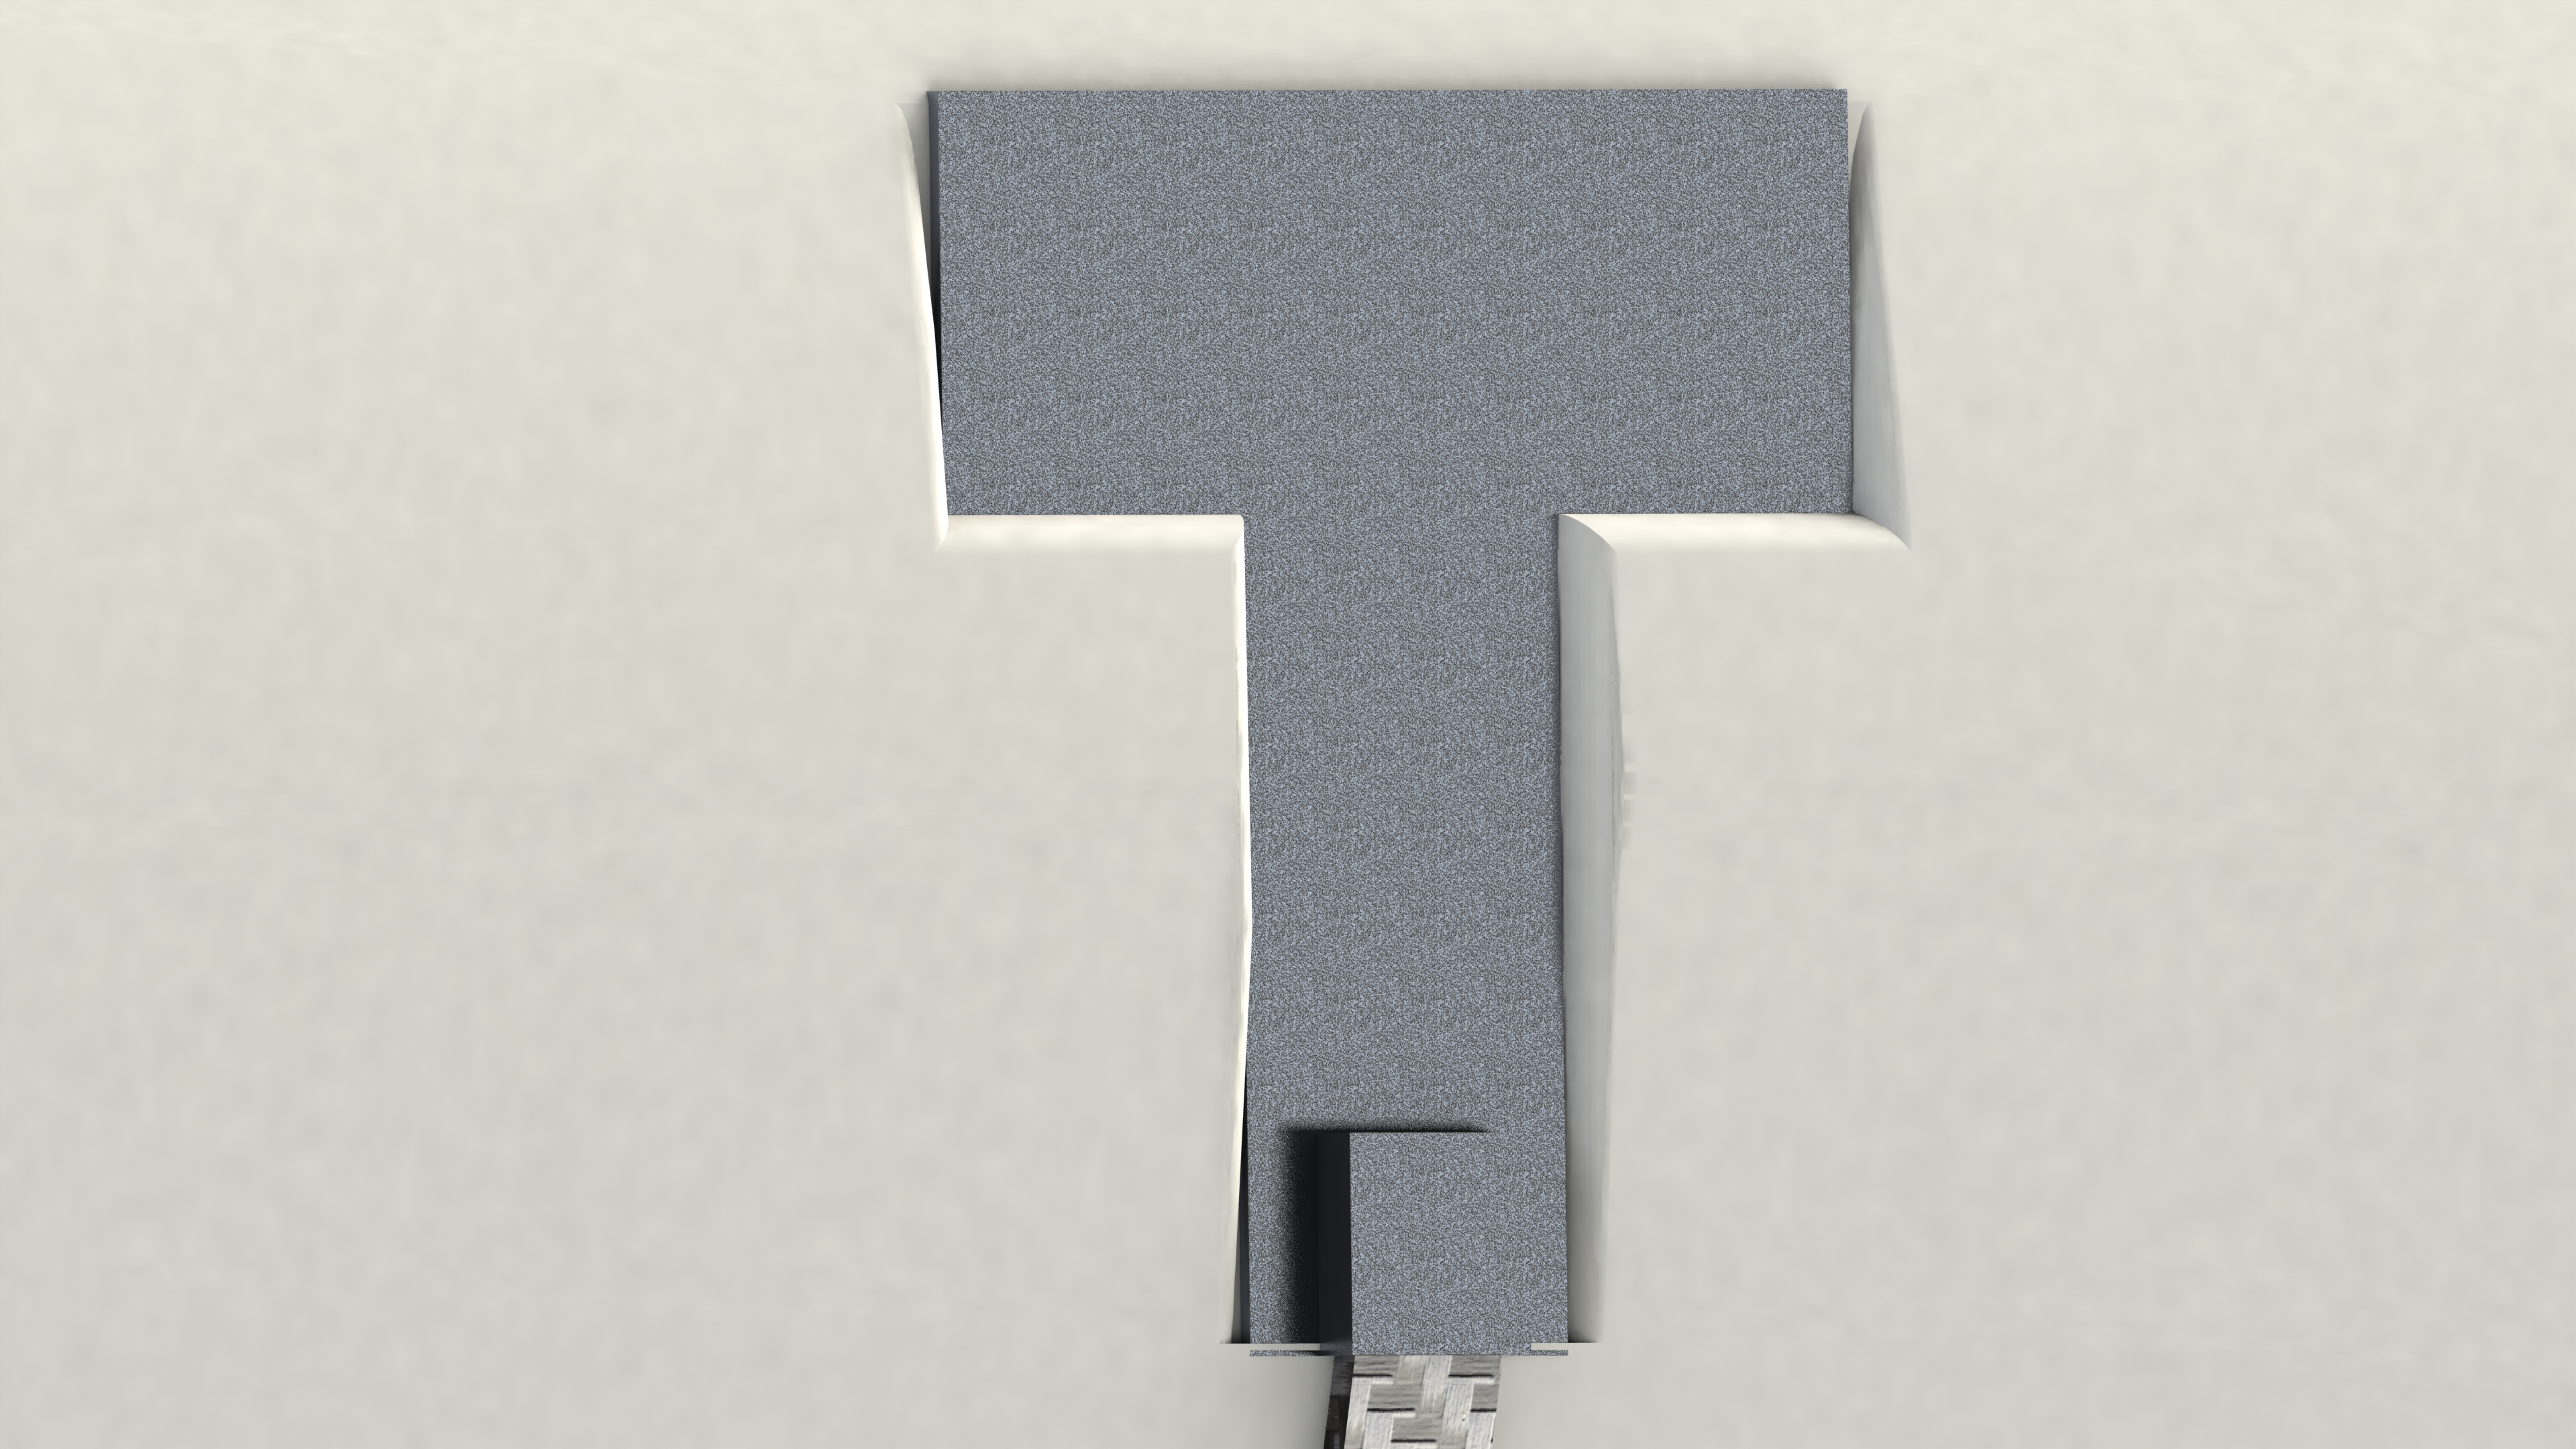
\includegraphics[width=.8\linewidth]{img/design/thruster/envelopeDeformation.JPG}
	\caption{Deformation of the Airship Envelope bt the Thruster Arms}
	\label{fig:envelopeDeformation}
\end{figure}

The compression will enable contact between the airship and plate, increasing the surface area for the double sided tape union. The edges of the aluminium plate will be bevelled to ensure that the plate does not pierce the envelope. All analysis performed in this report assumes that there is no support from the double sided tape at the plate, so that estimates of stresses are very conservative. The thruster arms will therefore be designed to sustain loading condition without support from the envelope.\\

The mounting of the plate to the thruster arm can be seen in Figure \ref{fig:thrusterOnKeel}. The full assembly can be seen in Figure \ref{fig:thrusterAssembly}.  

\begin{figure}[H]
	\centering
	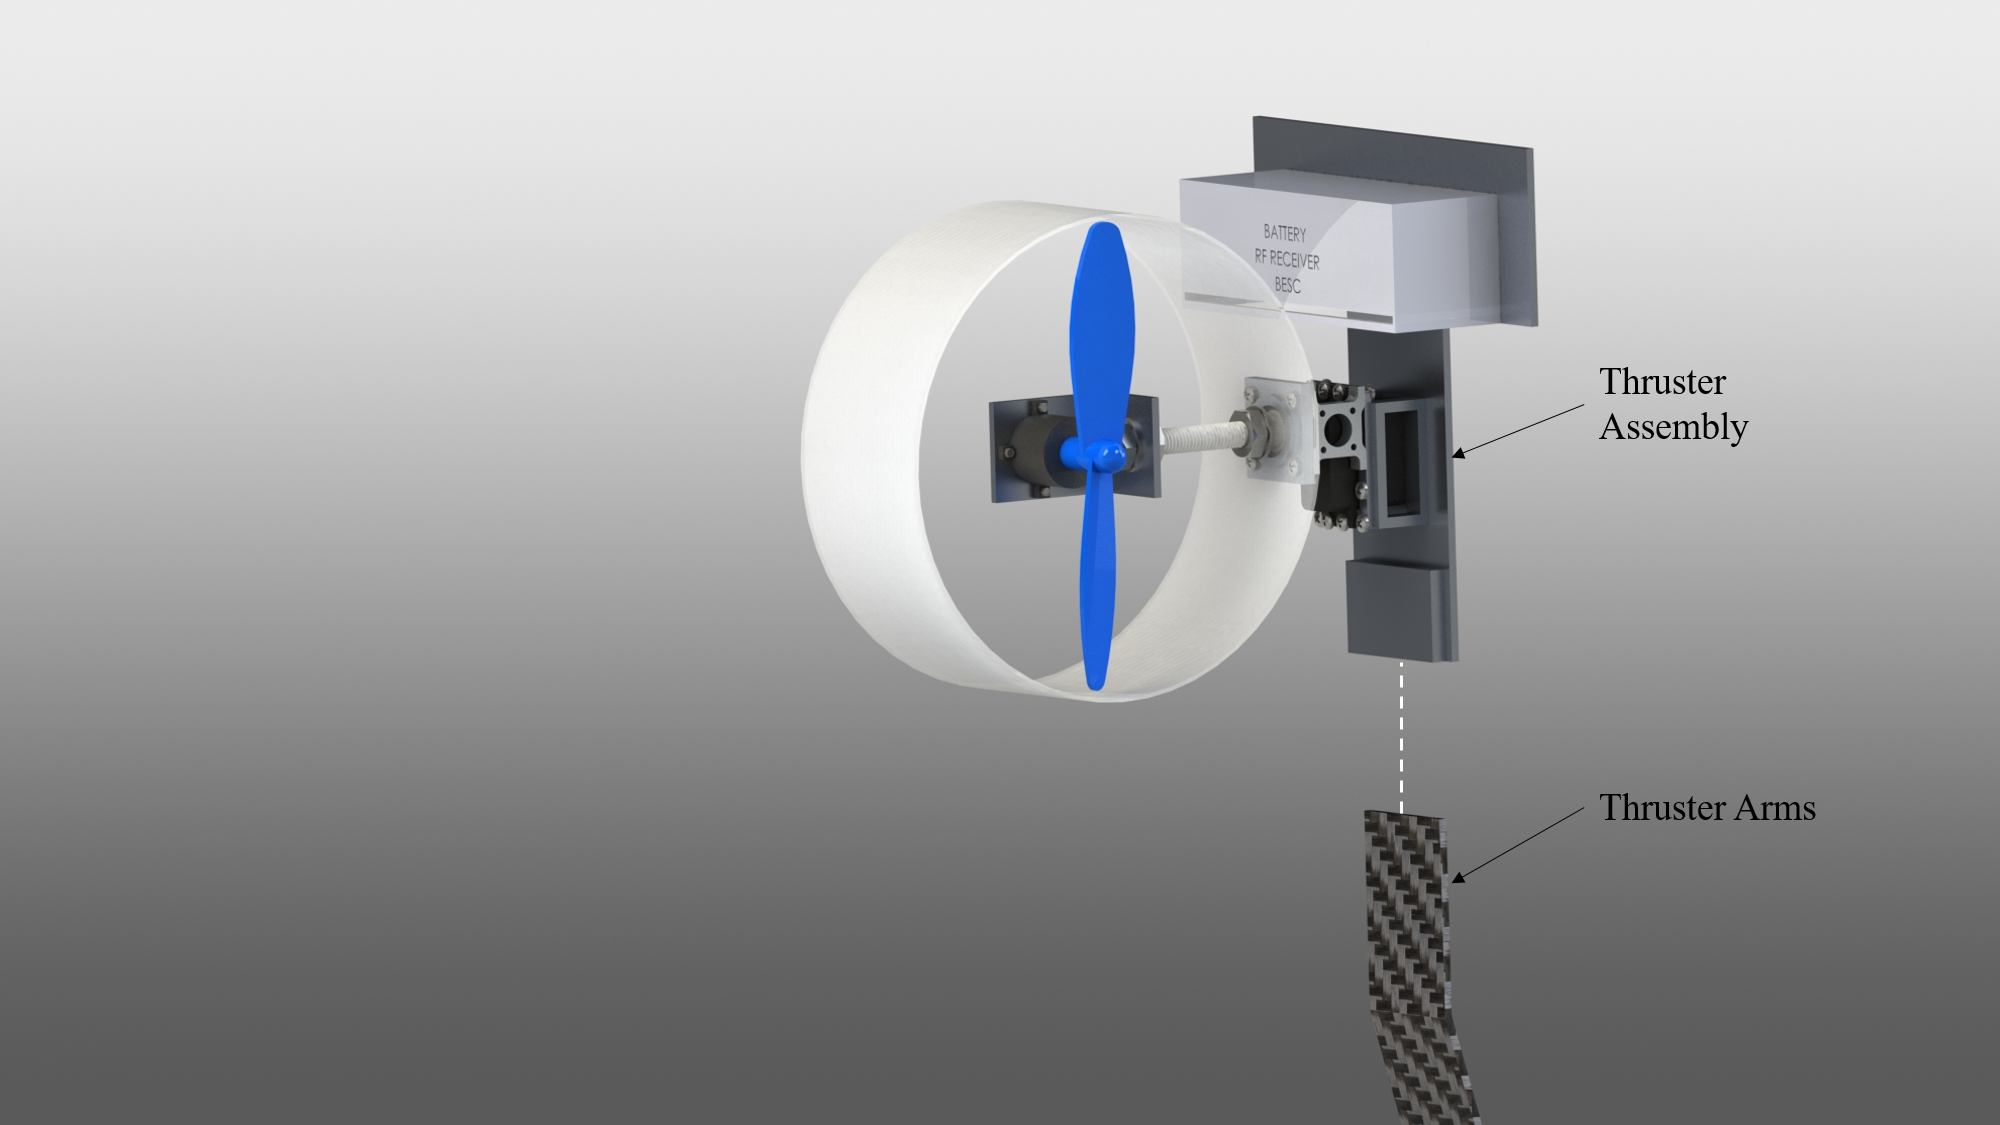
\includegraphics[width=.8\linewidth]{img/design/thruster/thrusterOnKeel.png}
	\caption{Thruster Assembly on Thruster Arm}
	\label{fig:thrusterOnKeel}
\end{figure}

Components are housed inside a 3D printed casing that features a 3D printed door, similar to that designed for the gondola. Figure \ref{fig:plateAssembly} displays how the components are mounted on the plate. The components for each thruster include a receiver, a battery and a BESC. The components are located above the centre of volume of the airship in the z-direction, raising the centre of mass, providing for better pitching properties. These components are well covered from the rain and any splashing water. The casing above the servo motor will shield it from rain in level flying conditions.

\begin{figure}[H]
	\centering
	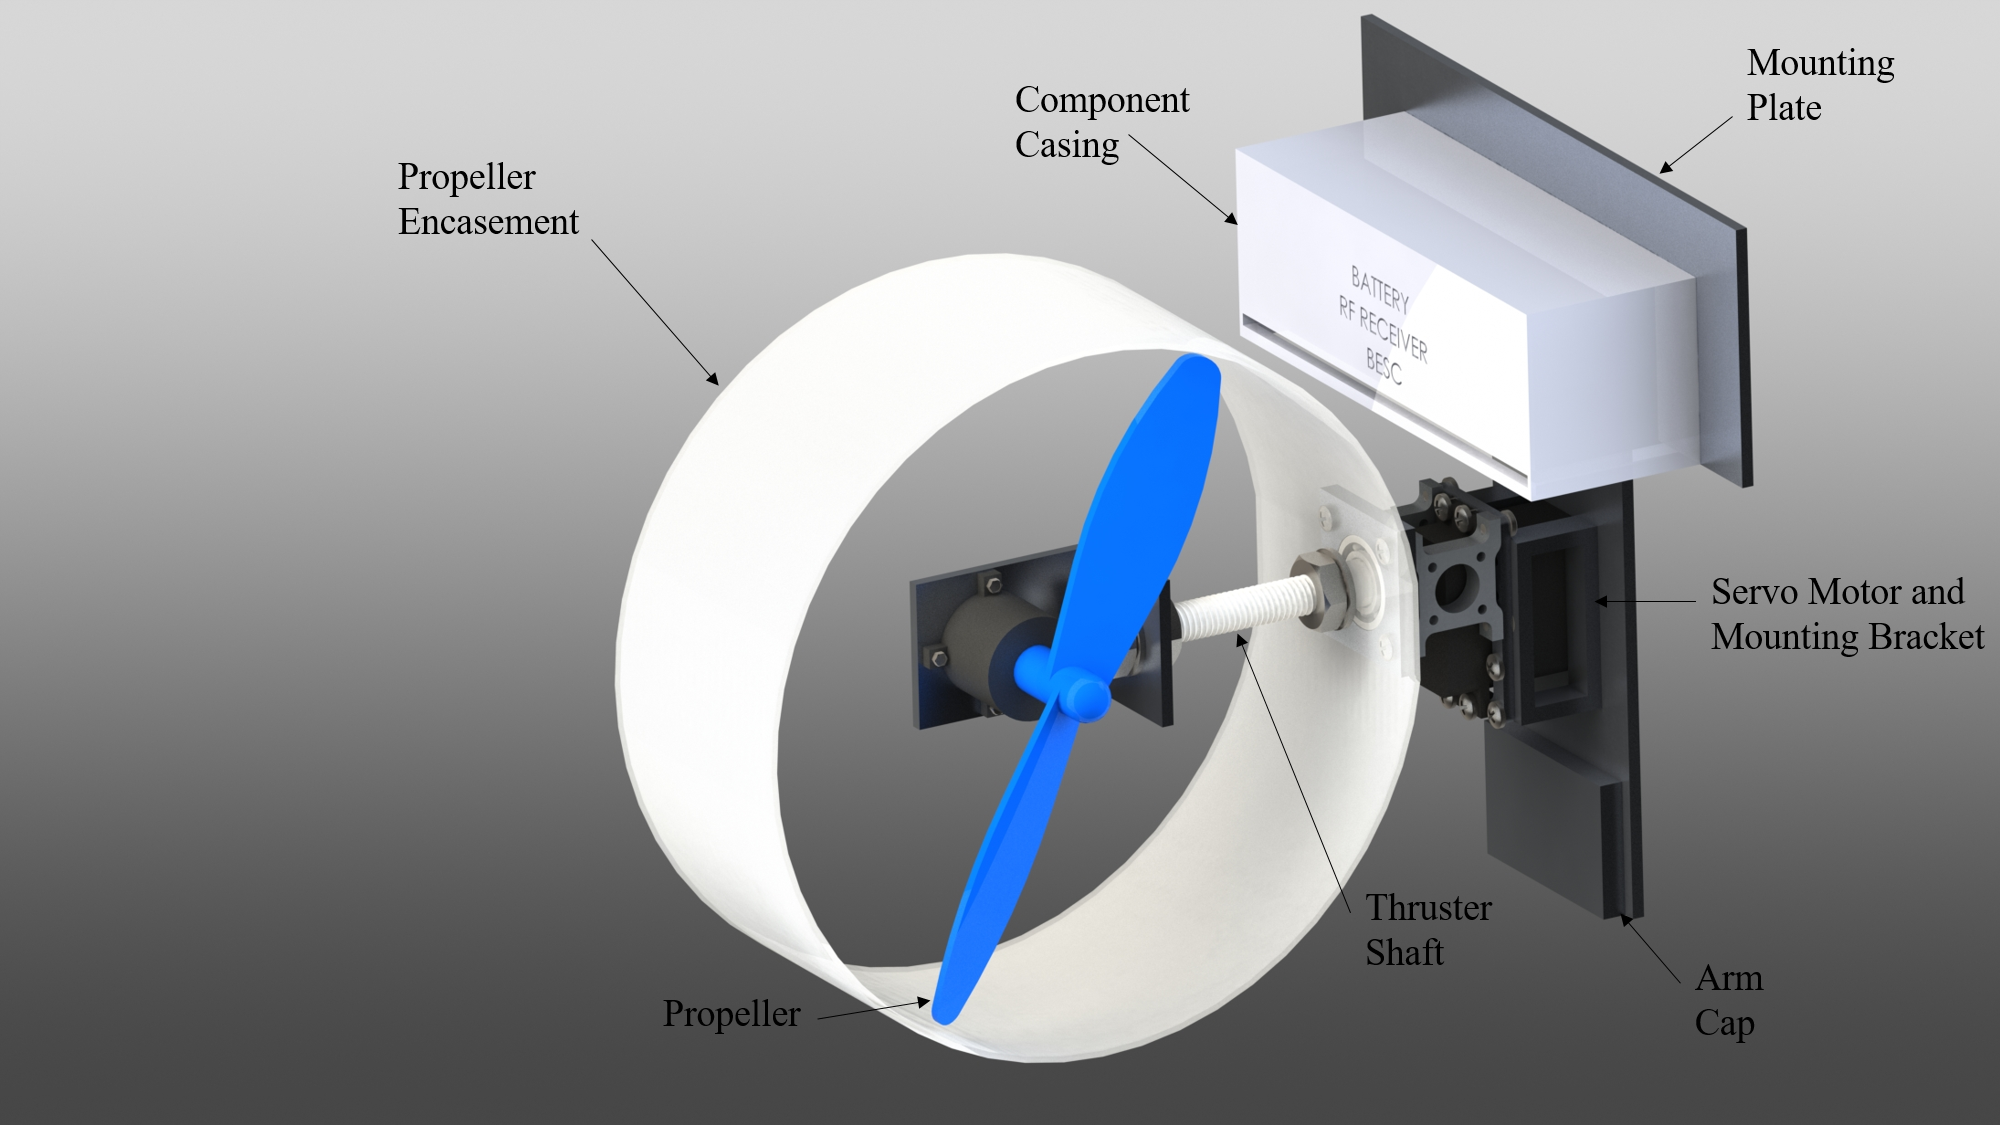
\includegraphics[width=.8\linewidth]{img/design/thruster/thrusterAssembly.png}
	\caption{Overall Thruster Assembly}
	\label{fig:thrusterAssembly}
\end{figure}


\begin{figure}[H]
	\centering
	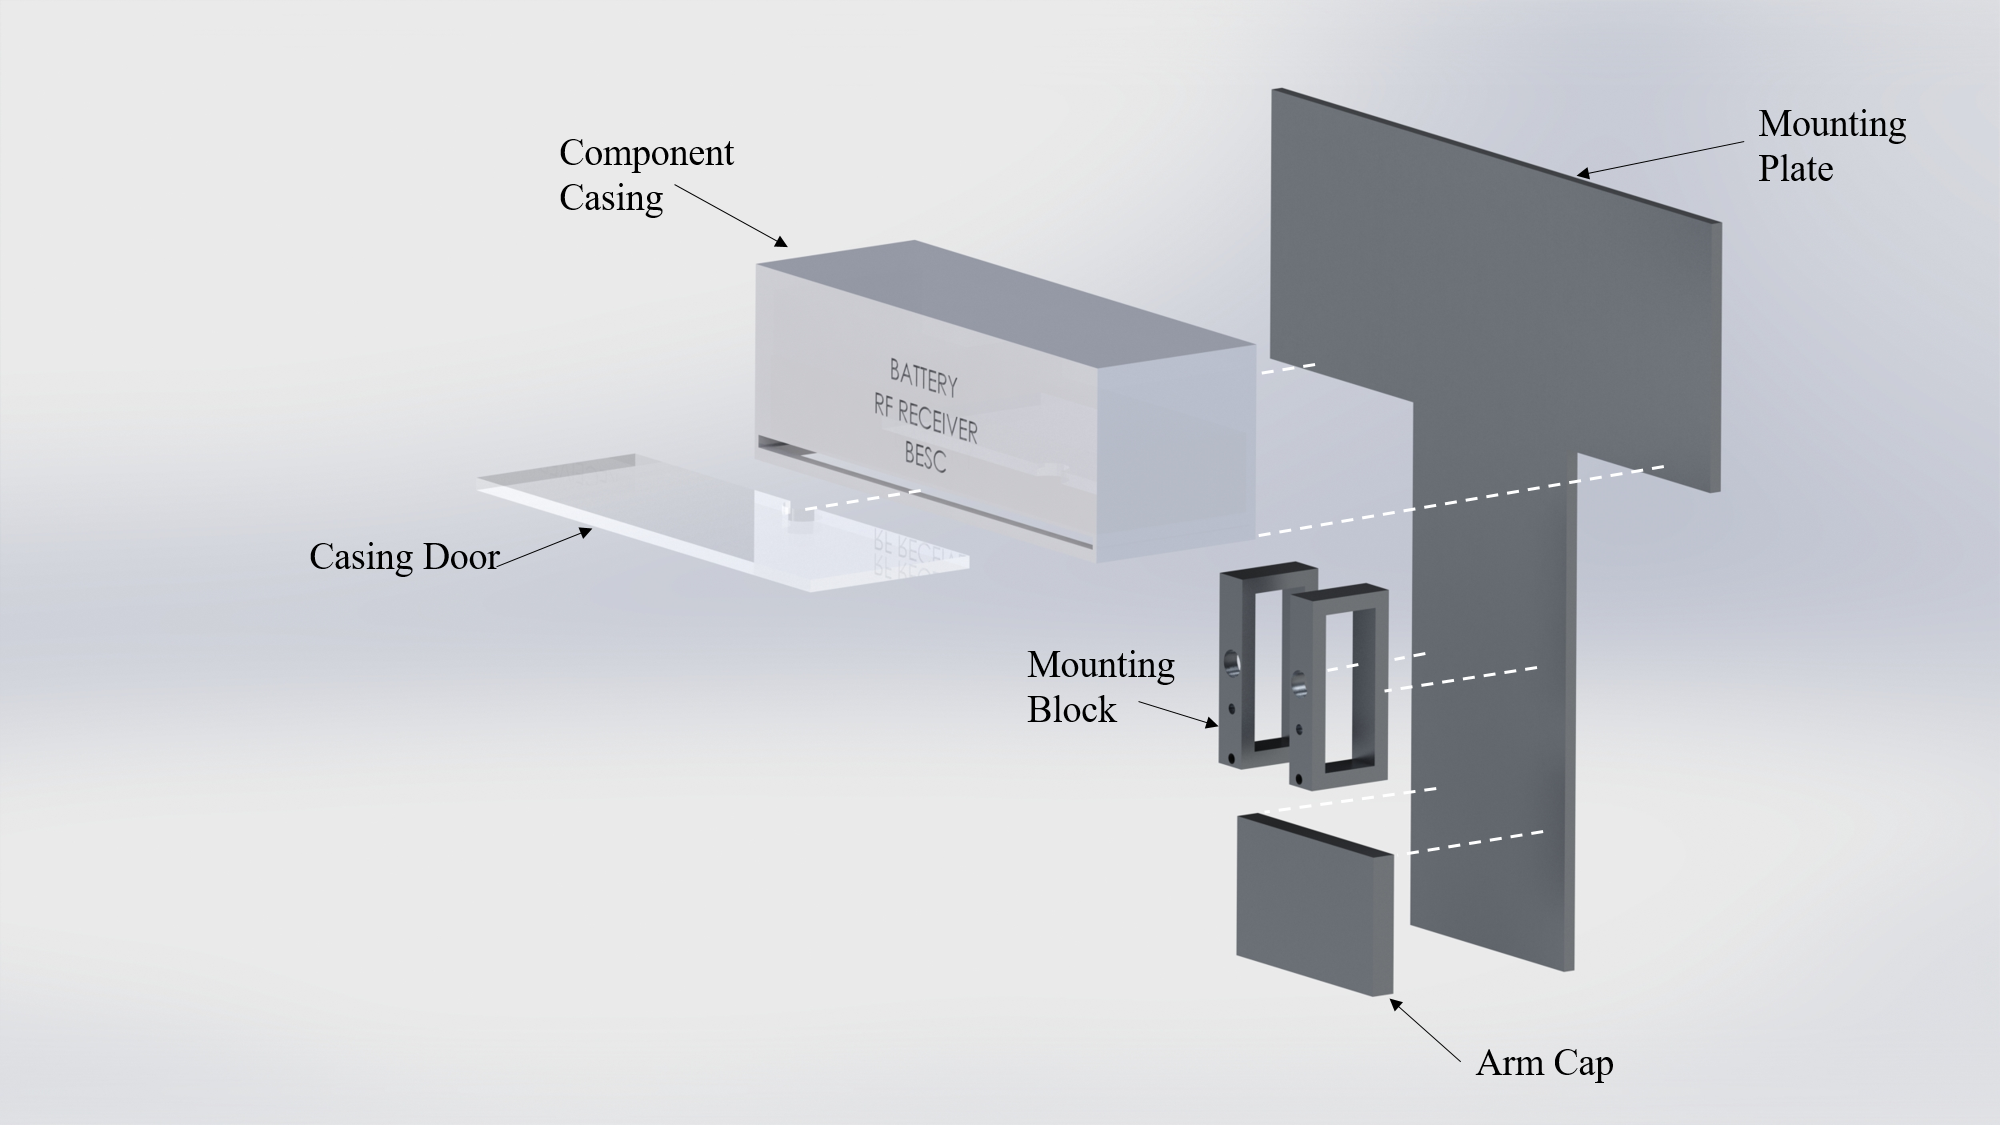
\includegraphics[width=.8\linewidth]{img/design/thruster/plateAssembly.png}
	\caption{Mounting Plate Exploded View}
	\label{fig:plateAssembly}
\end{figure}

 The servo motor is mounted to the plate using aluminium mounting blocks along with off-the-shelf assembly, as seen in Figure \ref{fig:servoAssembly}. The mounting blocks and arm cap are to be welded onto the mounting plate as shown in Figure \ref{fig:plateAssembly}.
 
  \begin{figure}[H]
 	\centering
 	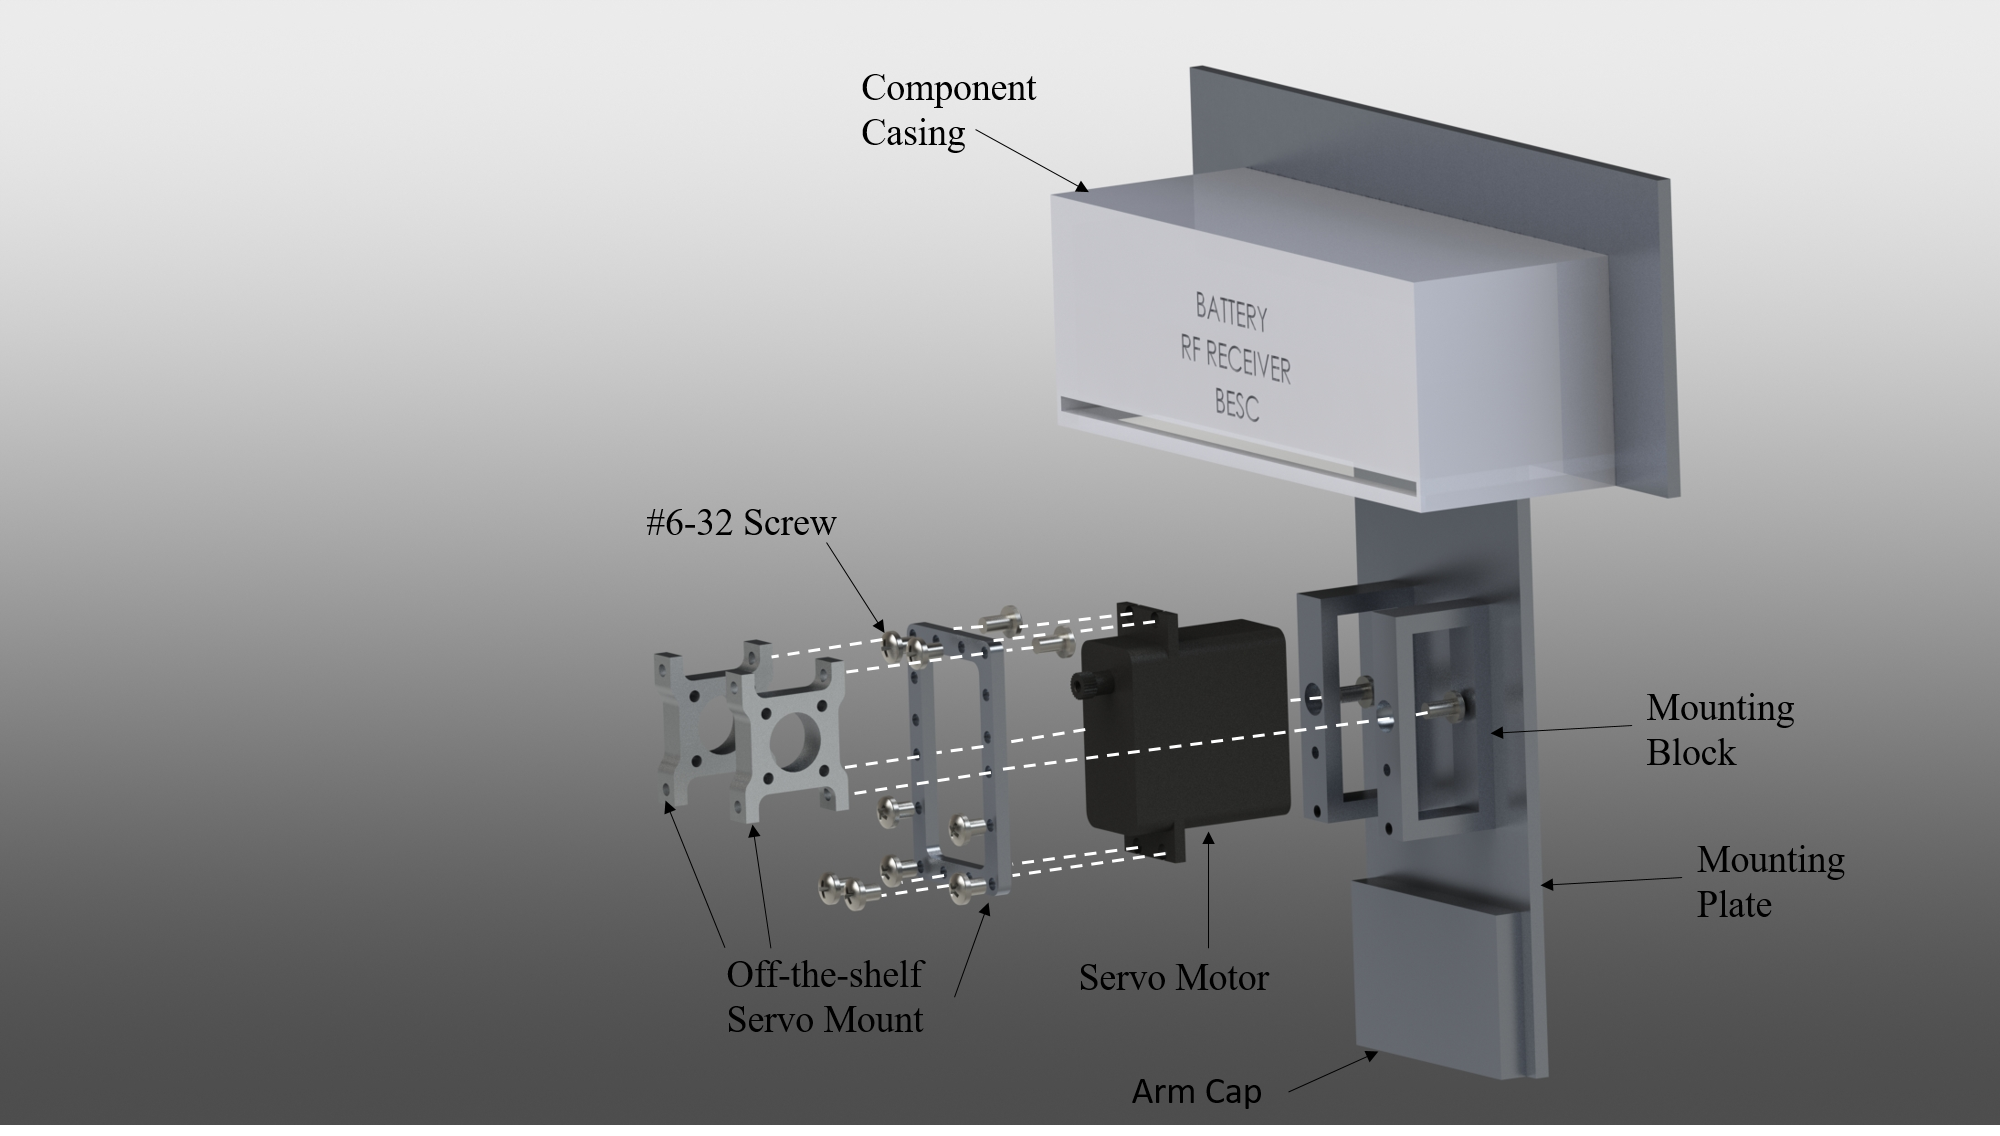
\includegraphics[width=.8\linewidth]{img/design/thruster/servoAssembly.png}
 	\caption{Servo Mounting Exploded View}
 	\label{fig:servoAssembly}
 \end{figure}
 
 A bearing and custom machined bracket are added to the off-the-shelf to support the shaft attached to the servo motor. Figure \ref{fig:shaftAssembly} shows the bearing bracket, bearing and shaft. The custom machined bracket features a shoulder to enable the shaft to support minimal and unexpected axial loads as well as to ease in the pressing of the bearing into the hub. Figure \ref{fig:bearingShoulder} shows the shoulder. 
 
   \begin{figure}[H]
 	\centering
 	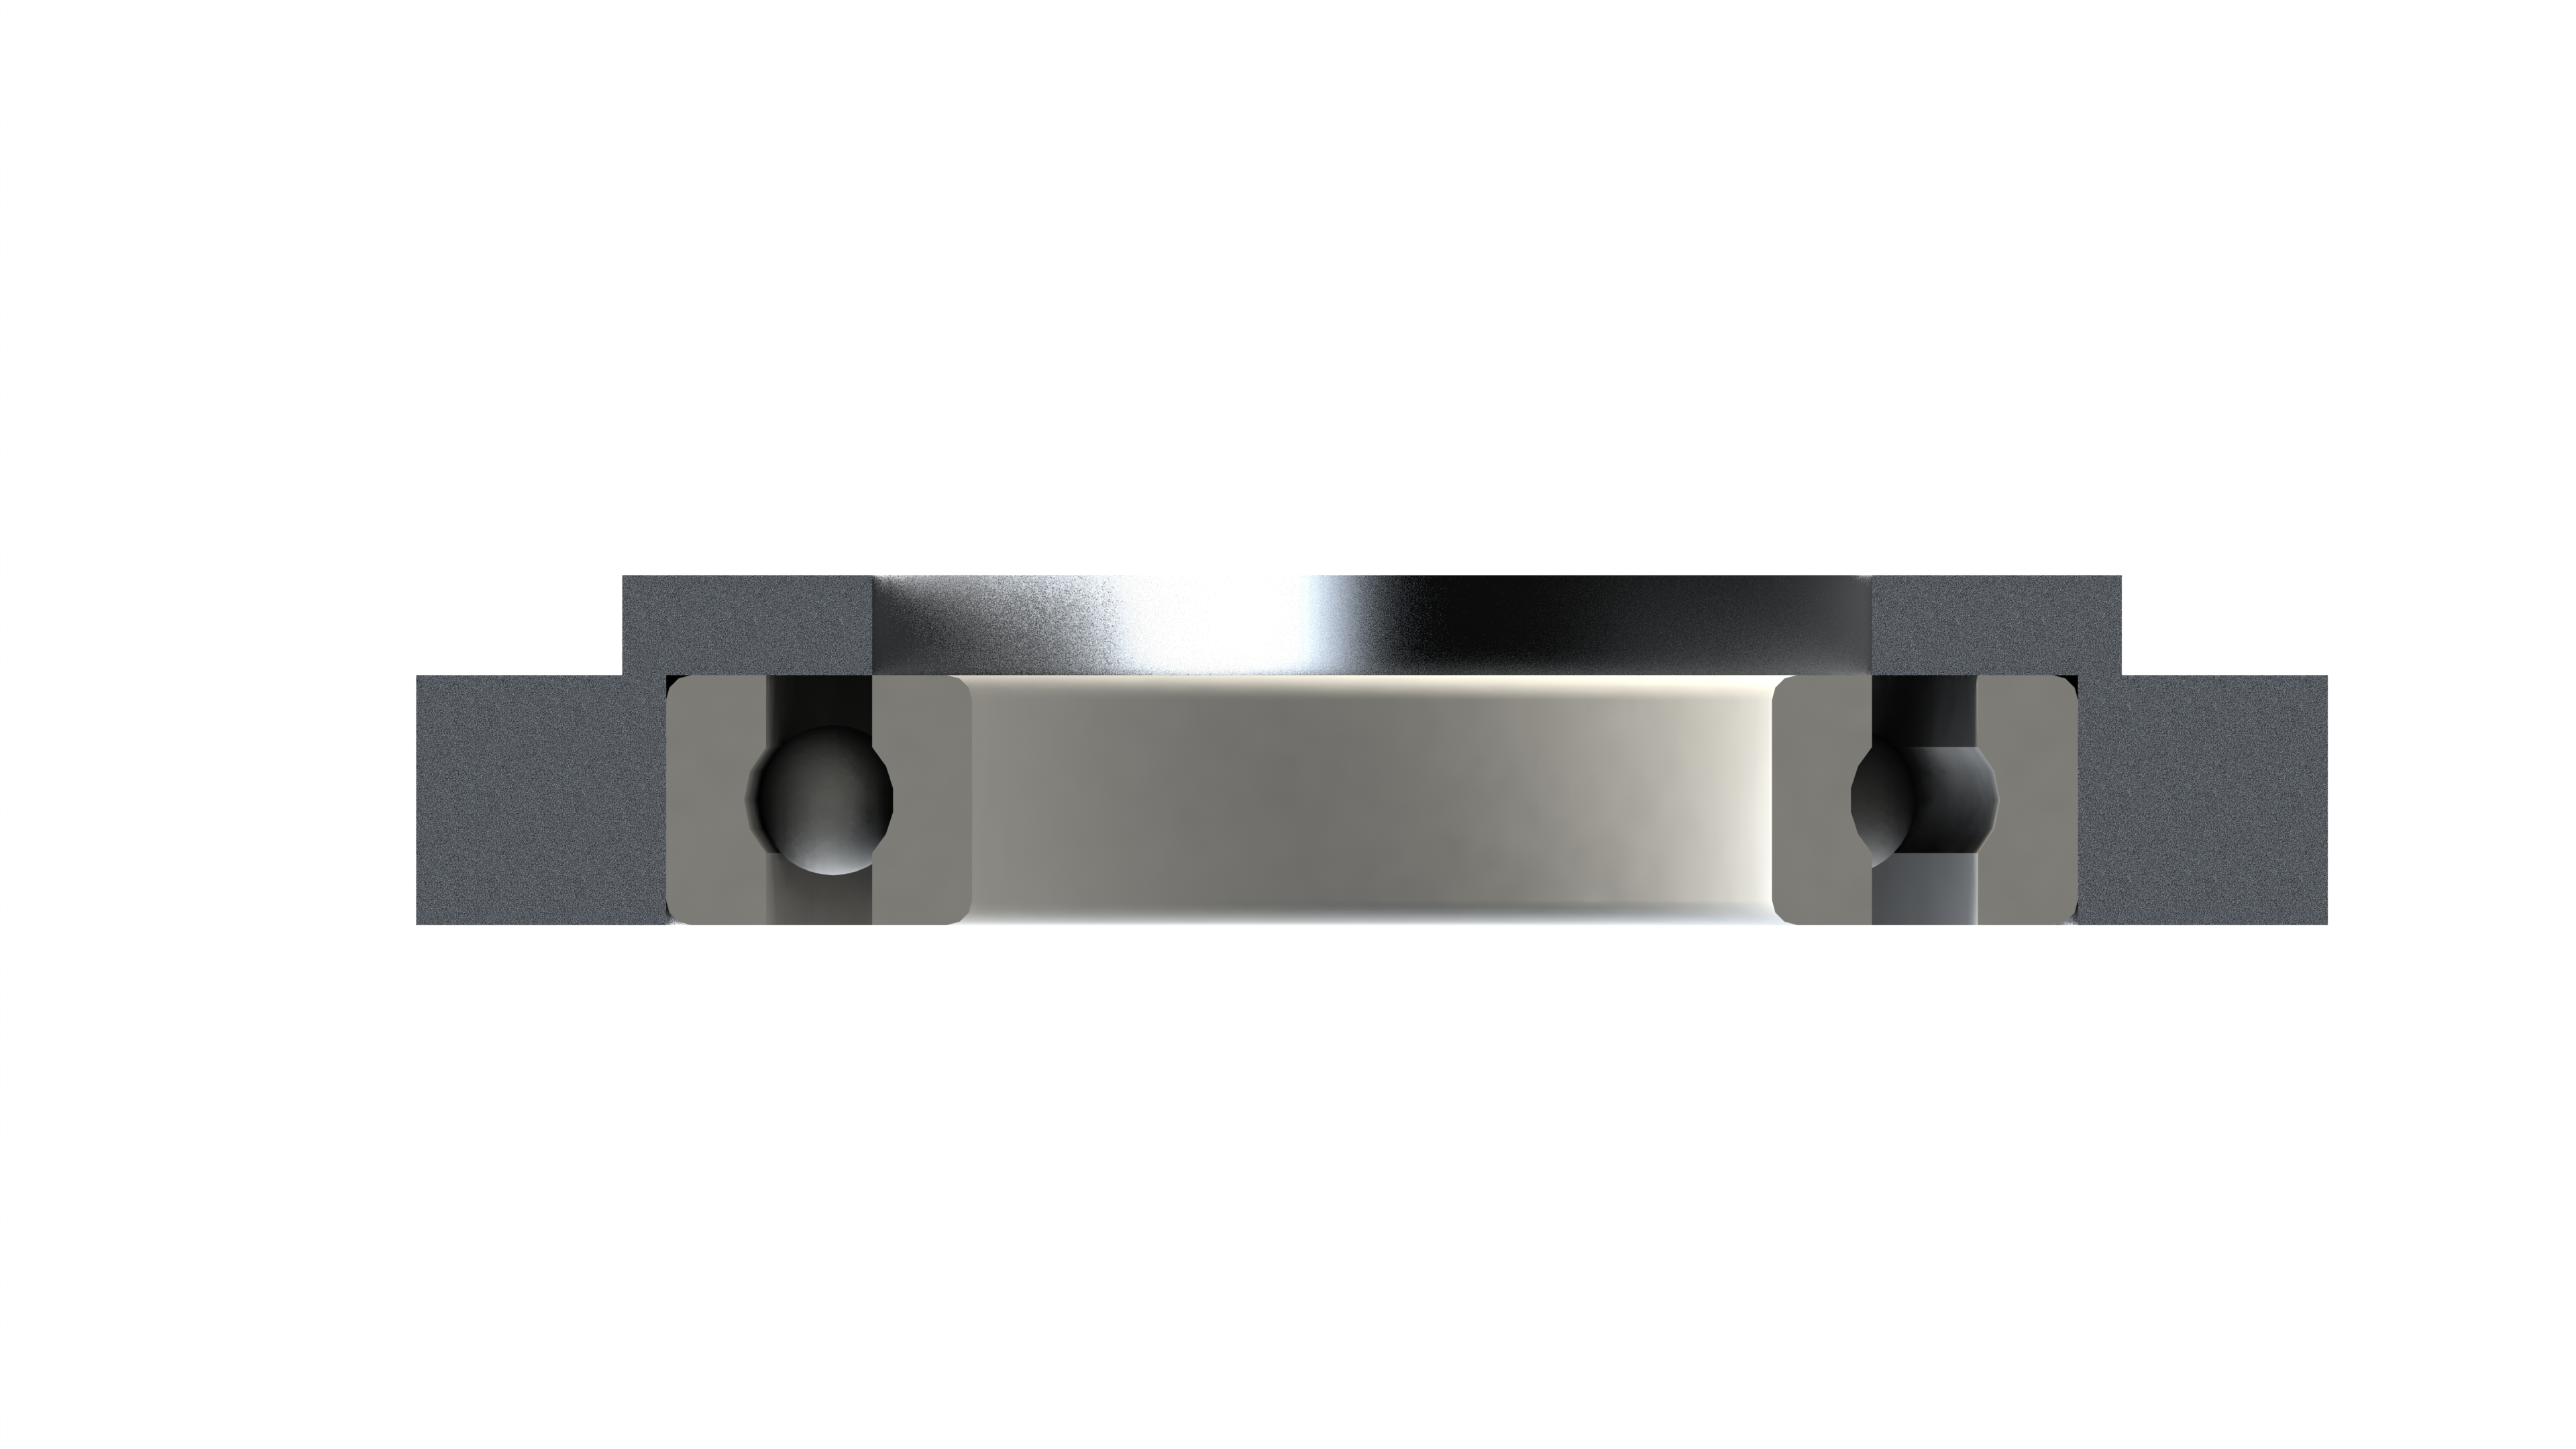
\includegraphics[width=.4\linewidth]{img/design/thruster/bearingLip.JPG}
 	\caption{Cross Section of Bearing Shoulder}
 	\label{fig:bearingShoulder}
 \end{figure}
 
 The shaft will be machined to be hollow and threaded on the outside. It will be manufactured using a Nylon 6, for its corrosion resistance, ease of machining, and low density. It will include a shoulder that fits into the bearing inner race. The shaft is mounted to the spline on the servo, and an M3 screw is placed inside to shaft, axially fastening it to the servo, that comes standard with a tapped hole. Several screws are used to securely fasten the servo to the supporting parts, all of which are shown in Figure \ref{fig:shaftAssembly}.
 
  \begin{figure}[H]
 	\centering
 	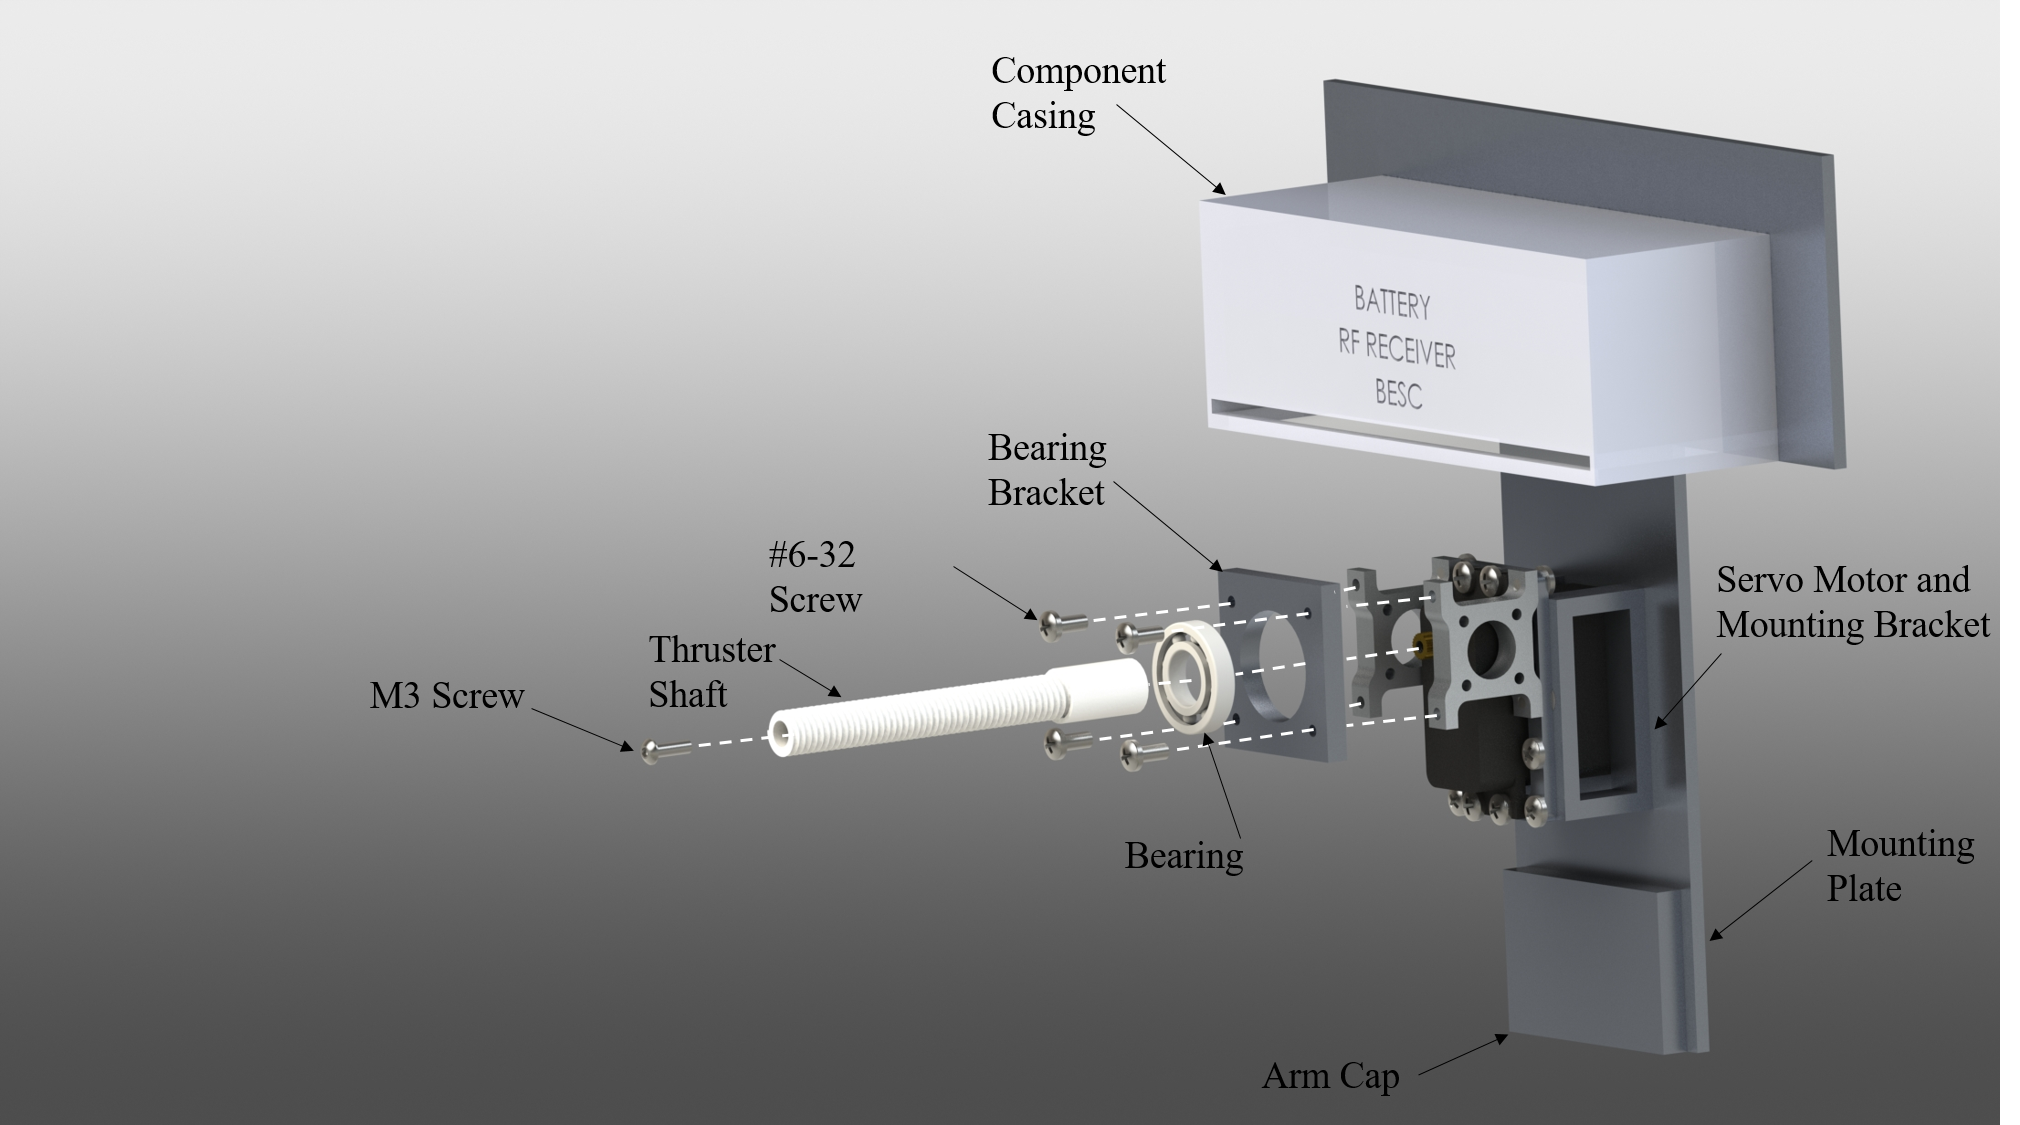
\includegraphics[width=.8\linewidth]{img/design/thruster/shaftAssembly.png}
 	\caption{Shaft Mounting Exploded View}
 	\label{fig:shaftAssembly}
 \end{figure}
 
The propeller motor is mounted on a machined aluminium propeller mounting bracket with tapped holes using screws, which is mounted on the shaft using washers and nuts, shown in Figure \ref{fig:mountAssembly}.

 \begin{figure}[H]
	\centering
	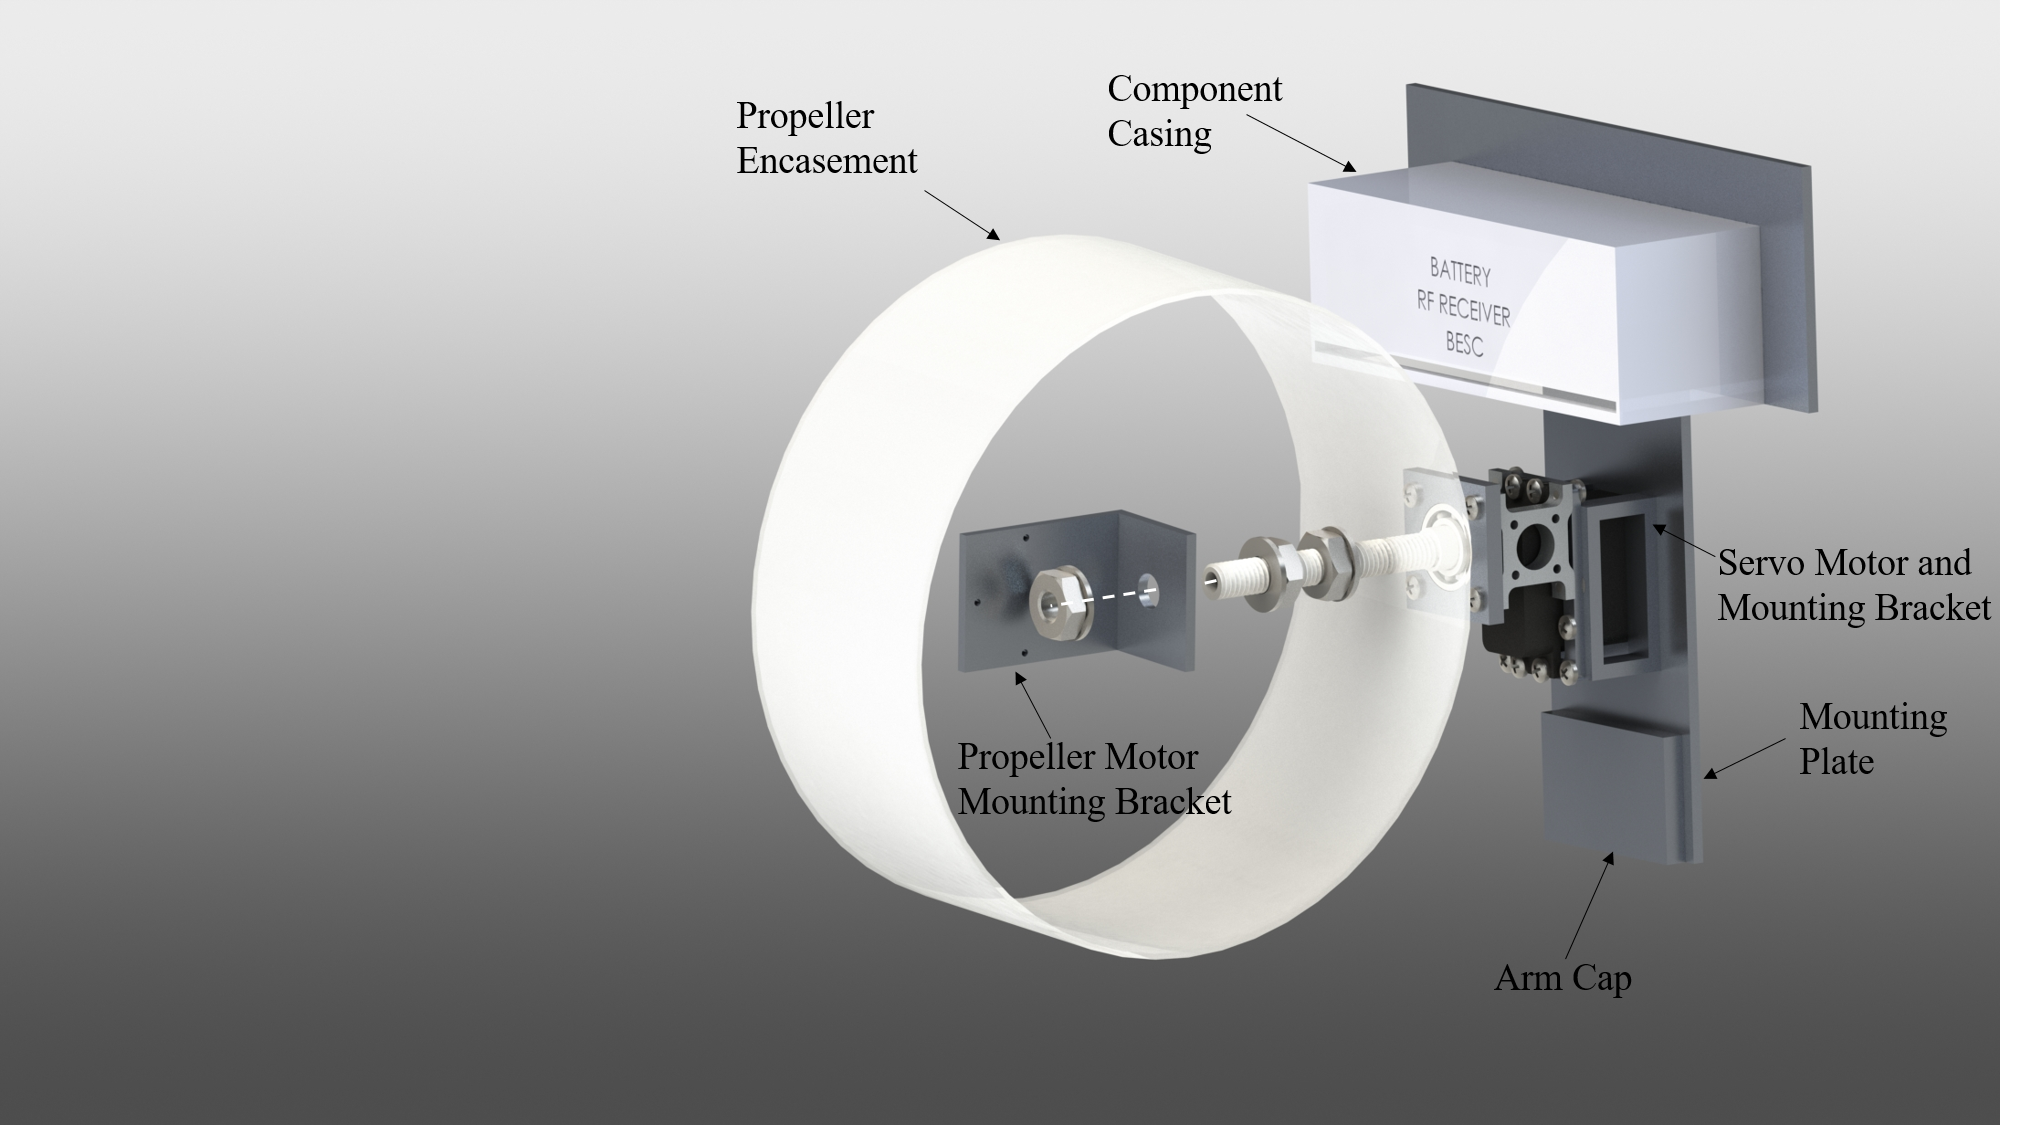
\includegraphics[width=.8\linewidth]{img/design/thruster/mountAssembly.png}
	\caption{Propeller Bracket Mounting Exploded View}
	\label{fig:mountAssembly}
\end{figure}

 Figure \ref{fig:propAssembly} shows how the propeller and related parts will be mounted. The propeller is mounted to the motor using a standard interference fit, given that these are both off-the-shelf parts. The propeller and motor are protected by a lightweight plastic encasement, cut from a sheet of transparent PETG (Polyethylene Terephthlate Glycol-Modified) plastic. The strip is formed to a loop and a hole is added, it is then mounted to the shaft by squeezing the plastic between a shoulder on the shaft and washer/nut combination. All washers and nuts on the Nylon shaft are also made of nylon. The encasement provides shielding of the propeller motor during forward flight conditions.

\begin{figure}[H]
	\centering
	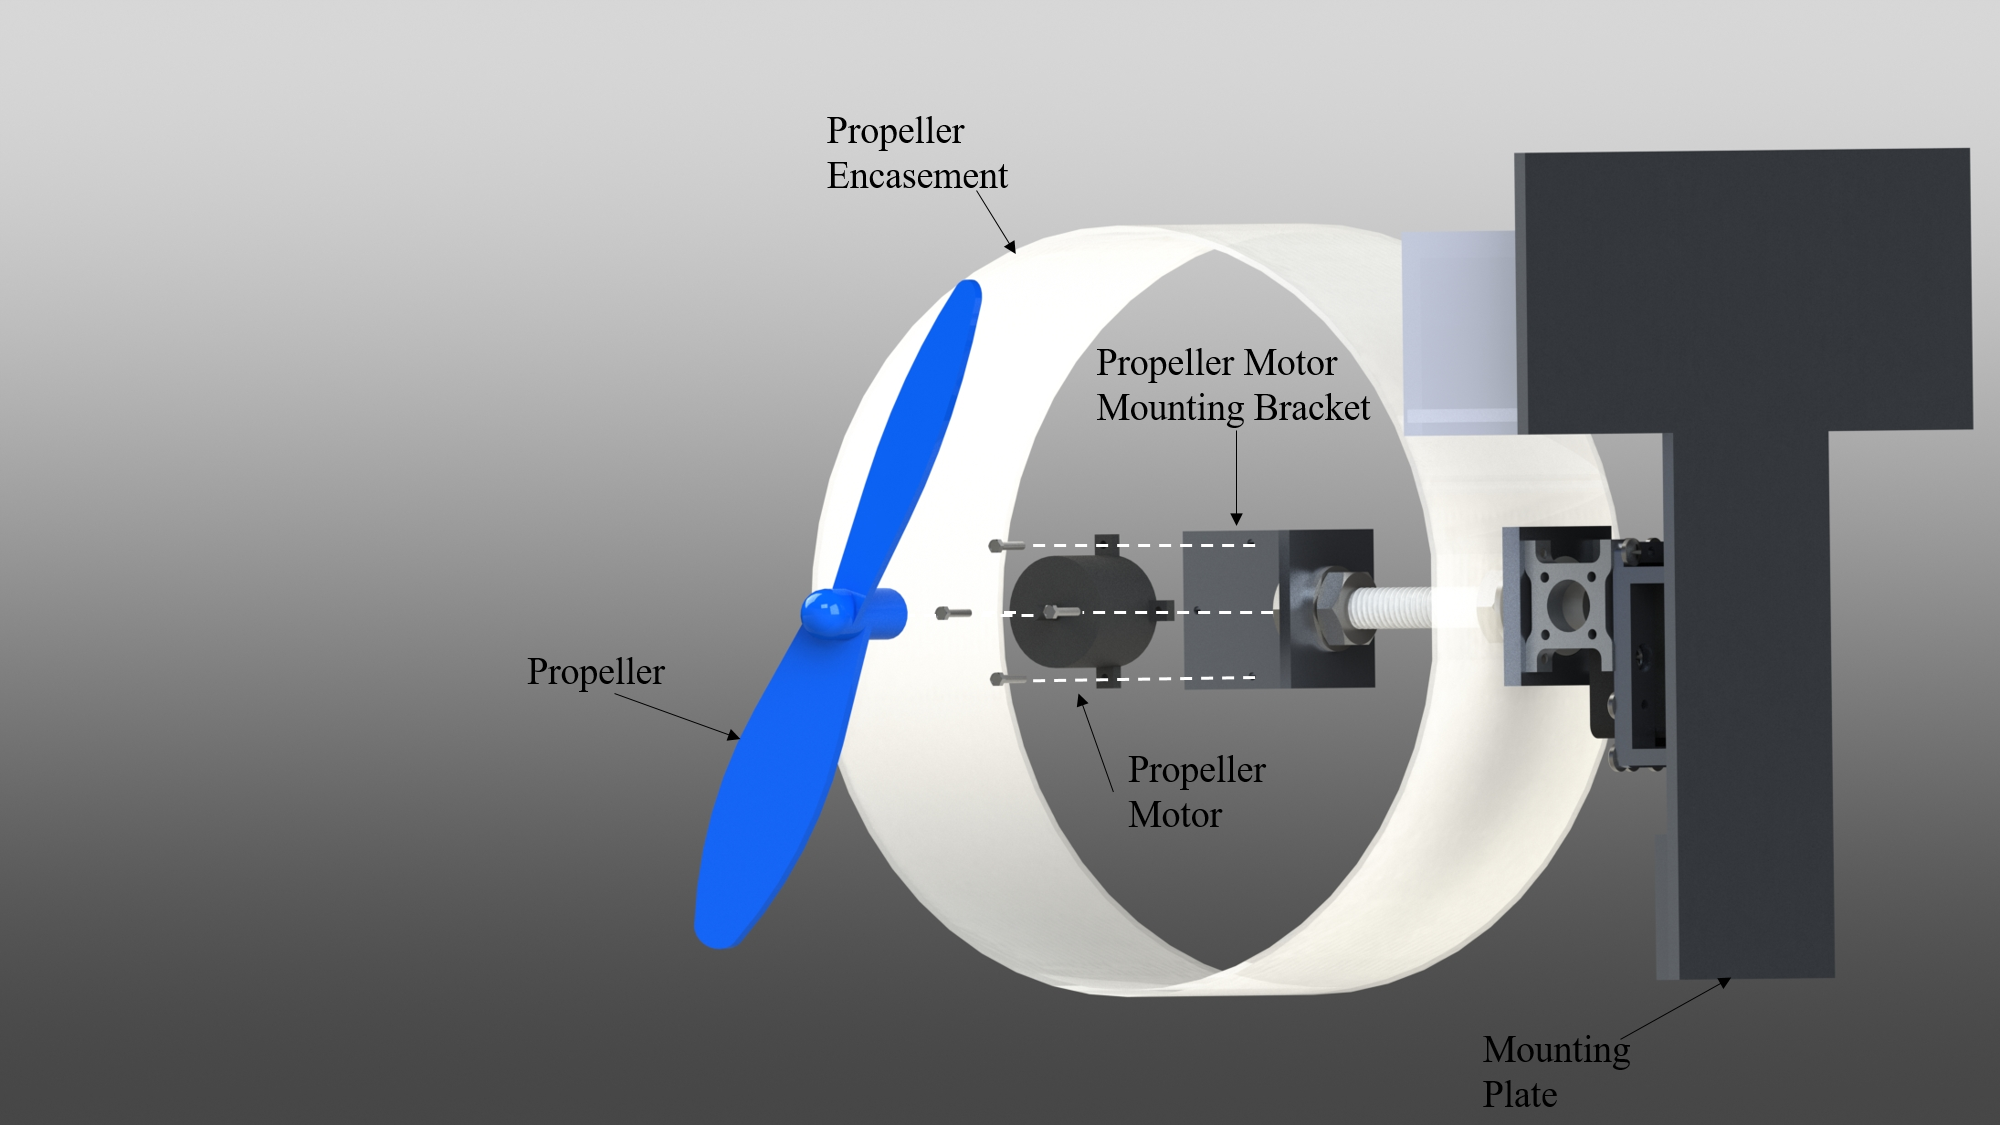
\includegraphics[width=.8\linewidth]{img/design/thruster/propAssembly.png}
	\caption{Propeller Exploded View}
	\label{fig:propAssembly}
\end{figure}

\section{Wiring and Weatherproofing}
Wiring for the airship is relatively straight forward as each motor assembly has an  independent power supply. Transmitters and receivers eliminate the need for wiring throughout the airship. Avoiding communication wiring significantly reduces the likelihood of wires tangling and jamming of parts. For the gondola, Figure \ref{fig:gondolaWiring} shows how wires will be routed. 

\begin{figure}[H]
	\centering
	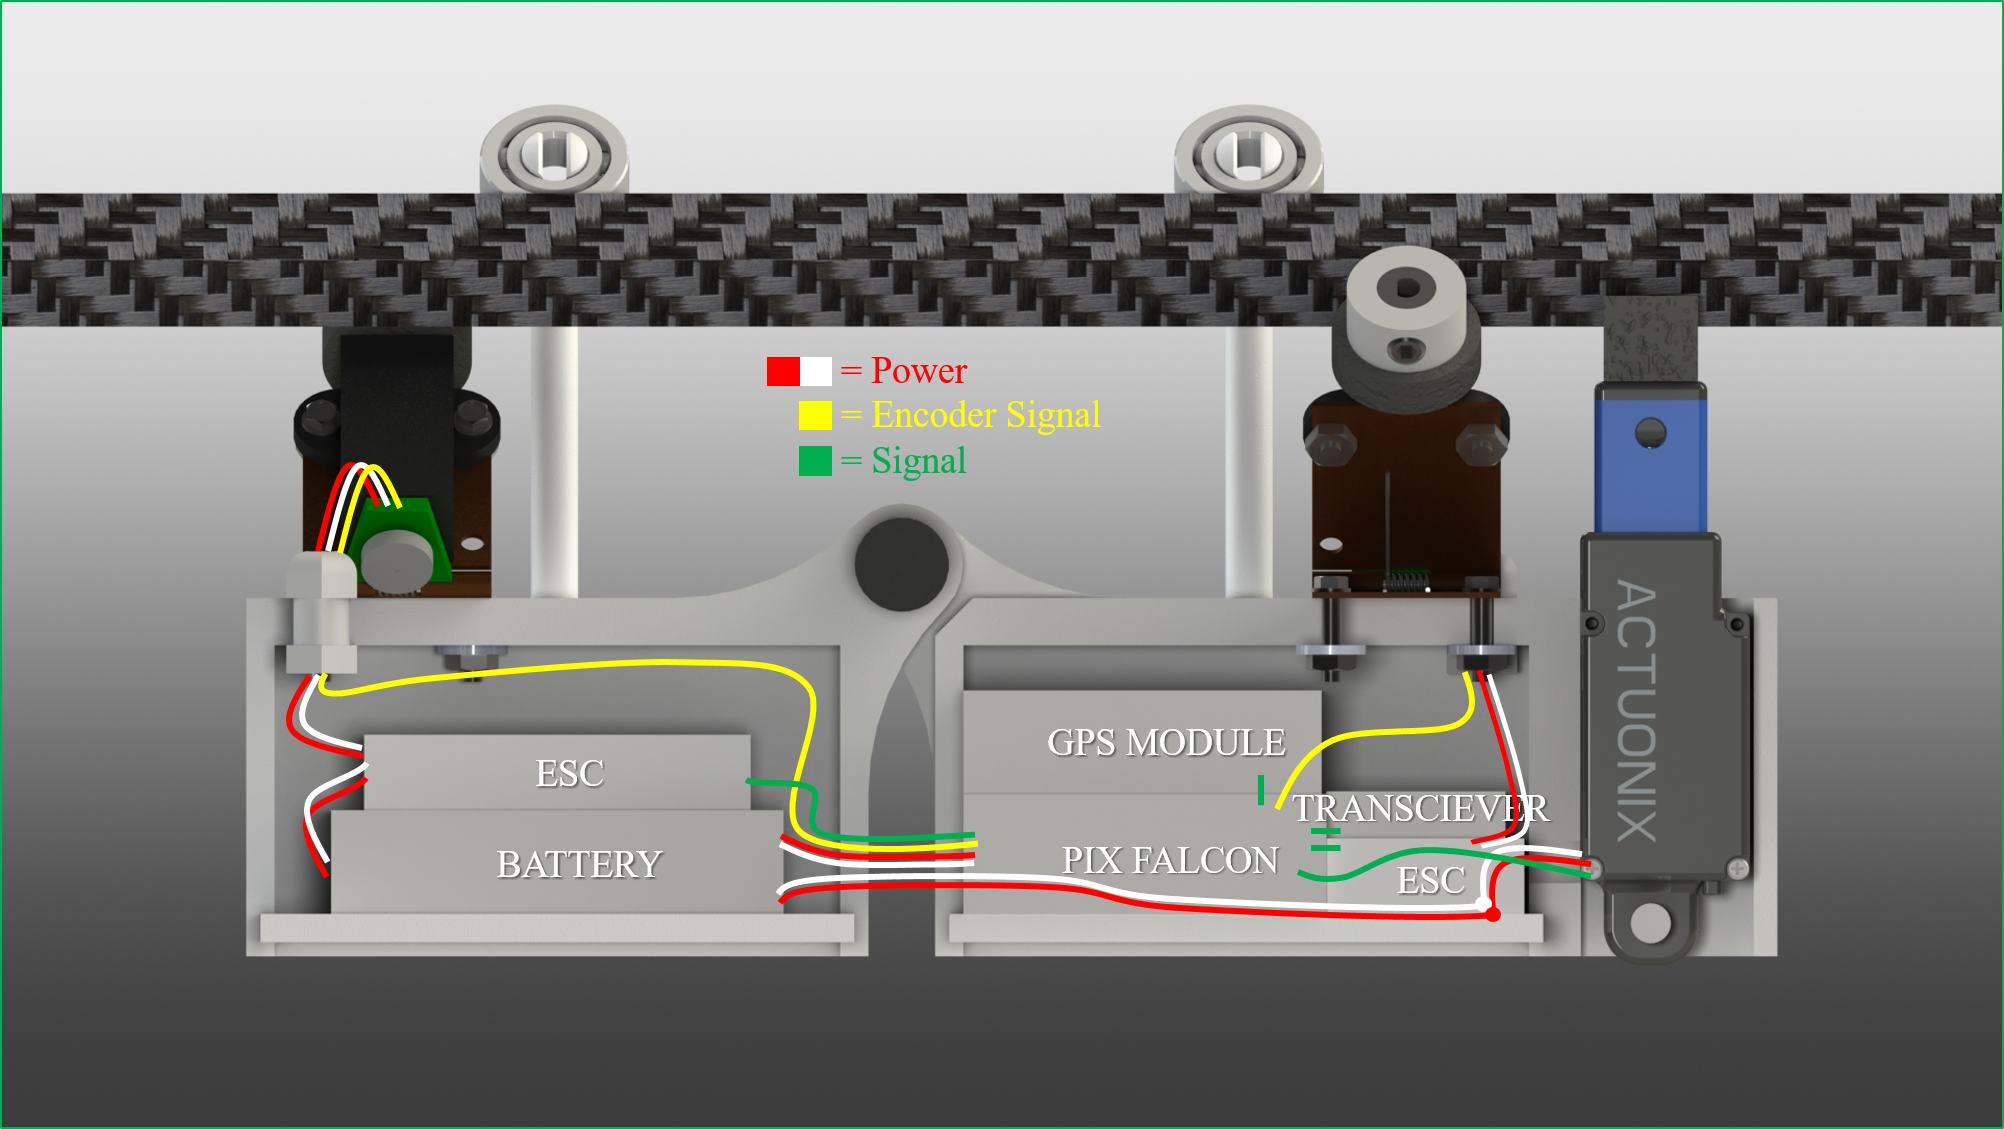
\includegraphics[width=.8\linewidth]{img/design/gondola/gondolaWiring.png}
	\caption{Gondola Component Wiring}
	\label{fig:gondolaWiring}
\end{figure}

Components shown are rough dimensions taken from the specifications for each part, and include the start of the tails of the wires, the size of the components in the figures are larger than the actual size of components. The figures look overcrowded for wiring, but the models are specifically oversized to account for room for wiring. Waterproofing is provided by cable glands for surfaces perpendicular to the fall of rain (see Appendix \ref{CableGland}). Surfaces parallel to the fall of rain do not have waterproofing as these are not exposed to much water. The wires routed between sections of the gondola will be provided with slack so the gondola can fold up to 10$^{\circ}$. Holes between the two gondola sections allow for the wires to be routed between them. A schematic of the gondola wiring can be seen in Figure \ref{fig:gondolaWiringSchematic}.

\begin{figure}[H]
	\centering
	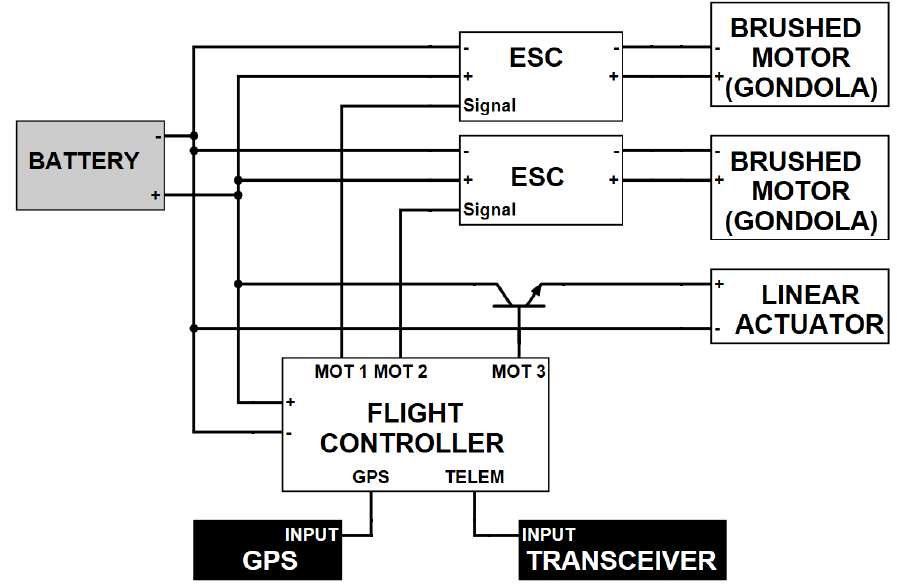
\includegraphics[width=.8\linewidth]{img/design/gondola/gondolaWiringSchematic.png}
	\caption{Gondola Component Wiring Schematic}
	\label{fig:gondolaWiringSchematic}
\end{figure}

The thruster assembly is wired similarly to the gondola, with wires coming out of the component casing. Most of the wiring is located inside the waterproof component casing. 2 sets of wires are routed out of the encasement: one to the vectoring motor, and one through the thruster shaft for the propeller motor. Figure \ref{fig:thrusterWiring} shows a diagram of the thruster wiring.

\begin{figure}[H]
	\centering
	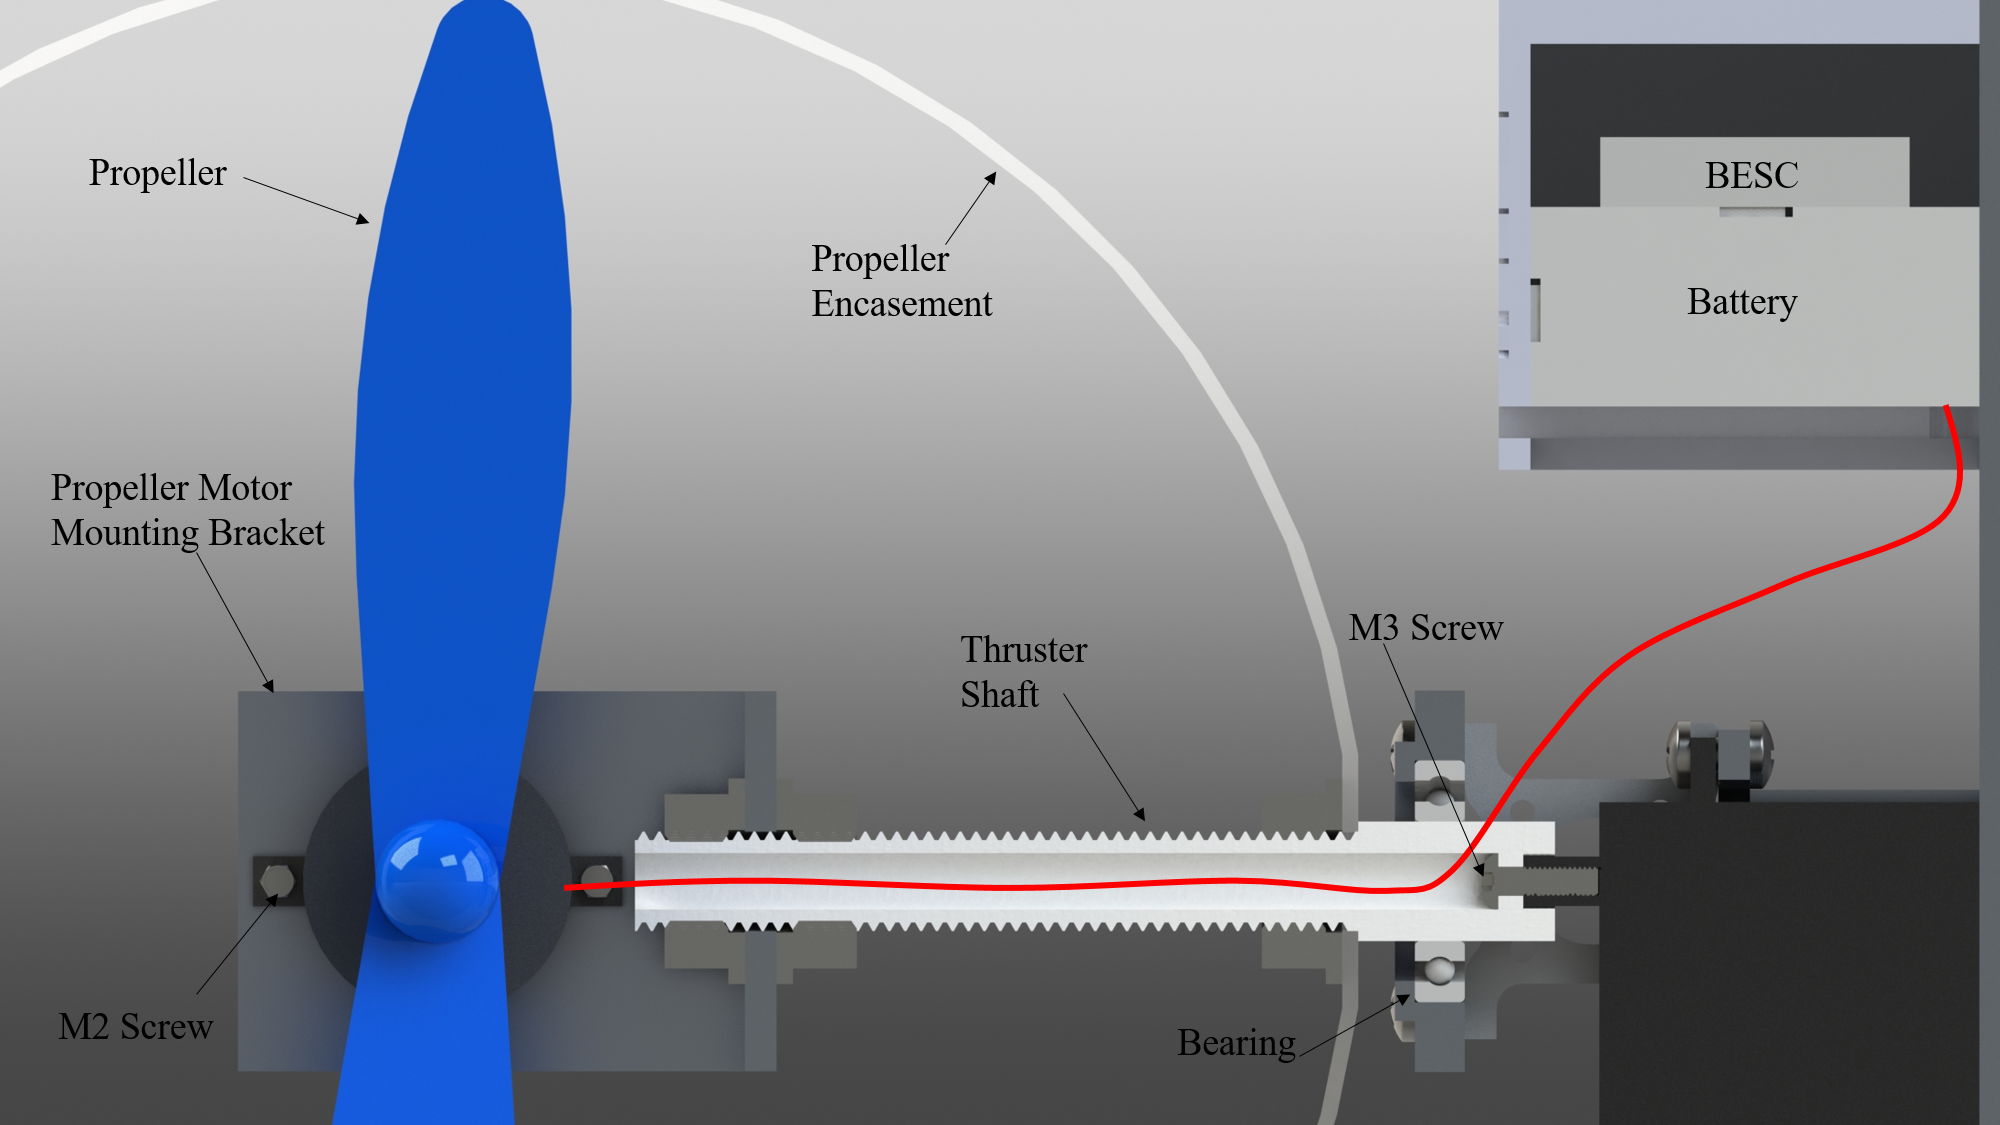
\includegraphics[width=.8\linewidth]{img/design/thruster/thrusterWiring.png}
	\caption{Thruster Wiring}
	\label{fig:thrusterWiring}
\end{figure}

 Waterproofing cannot be completed for the propeller motor as it must be exposed to the air to work and cool effectively. Although the propeller motor is not waterproofed, it is covered by falling rain by the propeller encasement in forward flight operations. A schematic of the wiring for the thruster assembly is shown in Figure \ref{fig:thrusterWiringSchematic}.

\begin{figure}[H]
	\centering
	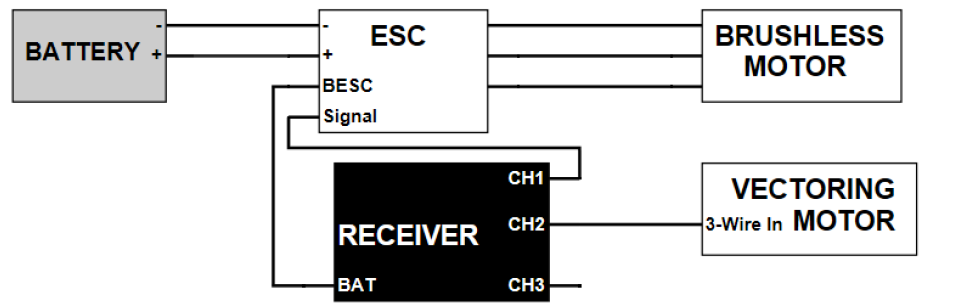
\includegraphics[width=.8\linewidth]{img/design/thruster/thrusterWiringSchematic.png}
	\caption{Thruster Wiring}
	\label{fig:thrusterWiringSchematic}
\end{figure}

All metal components are manufactured from aluminium, due to its relatively low weight as well as its resistance to corrosion.

\end{document}
